\chapter{IRK: Newtonen Iterazioa}
\label{chap:IRK-NEW}
%\epigraph{The top 10 algorithms in Applied Mathematics: 1.Newton and quasi-Newton methods.}
%{\textit {Nick Higham (2016)}}

\section{Sarrera}


Kapitulu honetan, Newtonen iterazioan oinarritutako IRK metodoen inplementazio eraginkorra ikertuko dugu.
Problema zurruna denean, puntu-finkoaren iterazioa ez da eraginkorra eta Newtonen iterazioa aplikatu behar da. Gainera problema ez-zurruna izanik ere, Newtonen iterazioak interesgarriak izan daitezke; bereziki doitasun altuko (doitasun laukoitza) konputazioetan iterazio metodoaren konbergentzia ezaugarri onak direla-eta. 

Ikusiko dugunez, $d$-dimentsioko ekuazio diferentzialen sistema, Newtonen iterazioan oinarritutako $s$-ataletako IRK metodoaren bidez integratzeko, era honetako ekuazio-sistema lineala askatu behar da
\begin{equation}
\label{eq:syslin}
(I_d \otimes I_s- h \ A \otimes J) \in \mathbb{R}^{sd \times sd},
\end{equation} 
non $A \in \mathbb{R}^{s \times s}$ Runge-Kutta metodoaren koefizienteen den eta $J$ matrizea, ataletan ebaluatutako matrize Jacobiarraren  hurbilpen komuna den. Integrazioaren urrats bakoitzean, $sd \times sd$ tamainako ekuazio-sistema lineala askatu behar da.

Hainbat lanetan \cite{Butcher1976,Liniger1970,Bickart1977}, (\ref{eq:syslin}) matrizearen egitura berezia aprobetxatuz, ekuazio-sistema linealak modu eraginkorrean ebazteko proposamena egin zuten. Zehazki, ia blokeka diagonala den (\ref{eq:syslin})~matrizearen antzekoa era honetako $I_d-h \lambda_j J \in \mathbb{R}^{d \times d} \ (j=1,\dots,s)$ $s$-bloke duen matrizea, bloke bat $A$ matrizearen $\lambda_j$ balio propio  bakoitzeko. Normalean, ordena altuko IRK metodoaren koefizienteen $A$ matrizeak, $[s/2]$ balio propio konplexu pare ditu ($s$ bakoitia denean, balio propio erreal bat gehituta).

Gure ekarpenean, $sd$-dimentsioko (\ref{eq:syslin}) ekuazio-sistema, $(s+1)d$~dimentsioko sistema gisa 
berridatziko dugu, eta $d \times d$ tamainako $[s/2]+1$ matrizeren LU deskonposaketa (eta tamaina bereko matrize batzuen biderketa) kalkulatuz, askatuko dugu. Tamaina txikiko matrizeen LU deskonposaketa azkarra denez, konputazionalki eraginkorra izatea espero dugu. Inplementazioa, IRK metodo simetriko eta sinplektikoetarako garatu dugu. Dena den, bai IRK metodo ez-simetriko sinplektikoetarako, bai IRK metodo simetriko ez-sinplektikoetarako garatu daiteke.
 
Newtonen iterazio metodoaren bidez, $u\in \mathbb{R}^{n}$ eta $F: \mathbb{R}^n \ \longrightarrow {\mathbb{R}}^n$ emanik, $F(u)=0$ betetzen duen $u^{[*]}$ soluzioa aurkitu nahi dugu. Hasierako soluzioaren $u^{[0]}$ estimazioa  emanik,  Newtonen iterazio sinplifikatuaren definizioa \ref{alg:nssg}~algoritmoan ikus daiteke.

\begin{algorithm}[H]
  \BlankLine
  $ \text{Hasieratu} \ \ u^{[0]}   \quad \quad \quad \quad \quad \quad \quad \quad\quad \quad \quad \quad \quad \quad \quad \quad \quad    (64-bit)$\;
  $M=LU(J) \ \ \quad \quad \quad \quad \quad \quad \quad \quad\quad \quad \quad \quad \quad \quad \quad \quad \quad    (32-bit)$\;
  \For{ (k=1,2,\dots \text{konbergentzia lortu arte})}
  {
   \BlankLine
   $F^{[k]}=F(u^{[k-1]}) \  \quad \ \quad \quad \quad \quad \quad \quad \quad \quad \quad \quad \quad \quad \ \   (64-bit)$\;
   $\text{Askatu} \ \ M \ \Delta u^{[k]}=- F^{[k]} \ \quad \ \quad \quad \quad \quad \quad \quad \quad \quad \ \ \  (32-bit)$\;
   \BlankLine
   $u^{[k]}=u^{[k-1]}+\Delta u^{[k]}  \ \ \ \quad \quad \quad \quad\quad \quad \quad \quad \quad \quad \quad \ \     (64-bit)$\;
  }
 \caption{Newton sinplifikatua}
 \label{alg:nssg}
\end{algorithm}
%
non $J \approx J(u^{[k]}) \in \mathbb{R}^{n \times n}$ matrize Jacobiarraren hurbilpena den,
\begin{equation*}
J(u^{[k]})=(J_{ij}(u^{[k]}))_{i,j}^n \ \text{non} \ J_{ij}(u^{[k]})=\partial F_i/\partial u_j (u^{[k]}), \ \ 1 \leq i,j \leq n. 
\end{equation*} 


Newton metodoaren eragiketa konplexuenak doitasun txikiagoan kalkula daitezke \cite{Baboulin20092526} eta honek, konputazionalki abantaila interesgarria suposatzen du. \ref{alg:nssg} algoritmoaren  eskuin aldean, inplementazioak erabilitako doitasuna $64$-biteko dela suposatuz, eragiketa bakoitzarentzat zein doitasun erabili beharko litzatekeen adierazi dugu; Jacobiarraren balioztapena eta aljebra linealeko eragiketak, doitasun arruntean ($32$-bit) kalkulatu daitezke. Horrela konputazio denbora azkartuko litzateke.

Newtonen iterazioan oinarritutako IRK metodoen azterketa, era honetan egituratu dugu. Lehenengo, (\ref{sec:7.2}) atalean, Newtonen iterazio estandarraren azalpenak eman ditugu eta notazioa finkatu dugu. (\ref{sec:7.3}) atalean, Newtonen iterazioen ekuazio-sistema modu eraginkorrean askatzeko teknika deskribatu dugu. Hurrengo, (\ref{sec:7.4})-(\ref{sec:7.5}) ataletan, Runge-Kutta metodoen formulazio berriarekin aplikatzeko zehaztasunak eman ditugu. (\ref{sec:7.6}) atalean, Newtonen iterazioan oinarritutako IRK metodoaren inplementazio berria aurkeztu dugu. Azkenik, (\ref{sec:7.7}) atalean, inplementazio berriarekin egindako zenbakizko esperimentuen emaitzak eman ditugu. 

\section{IRK-Newton estandarra}
\label{sec:7.2}

Demagun honako hasierako baliodun problema,
\begin{equation}
\label{eq:hbp}
\dot{y}=f(t,y),\ \ \ y(t_0)=y_0, 
\end{equation}
non  $y_0 \in \mathbb{R}^{d}$  eta $f: \  {\mathbb{R}}^{d+1} \ \longrightarrow {\mathbb{R}}^d$ diren. 

Denbora diskretizazioa $t_0<t_1<t_2<\dots$ emanik, (\ref{eq:hbp}) hasierako baliodun problemaren $y(t)$ soluzioaren $y_n \approx y(t_n), (n=1,2,\dots)$ zenbakizko soluzioa, integrazio metodo bat aplikatuz lortuko dugu:
\begin{equation}
y_{n+1}=\Phi(y_n, t_n, t_{n+1}-t_n),
\end{equation}
non $\Phi:\mathbb{R}^{d+2} \rightarrow \mathbb{R}$ den.

S-ataletako IRK metodoaren kasuan,  $a_{ij}, b_i, \ \text{eta} \ c_i \ (1\leqslant i,j \leqslant s)$ koefizienteek definitzen dute $\Phi$ integrazio metodoa,
\begin{equation}  
\label{eq:irkn1}
\Phi(y,t,h)=y+h\sum^s_{i=1}{b_i \ f(t+c_ih,Y_{i})\ \ },\
\end{equation} 
%
non $c_i=\sum_{j=1}^{s} a_{ij}$ izan ohi den eta $Y_{i}$ atalak era honetan inplizituki  definitzen diren,
\begin{equation}
\label{eq:irkyi}
Y_{i}=y+\ h\ \sum^s_{j=1}{a_{ij}\ f(t+c_jh,Y_{j})}\ \ \ \ \ i=1 ,\dots, s.\
\end{equation} 

(\ref{eq:irkn1}) kalkulatu ahal izateko, $Y_{i} \in \mathbb{R}^d,\ i=1,\ldots,s$ ezezagunak lortu behar ditugu. Bakoitza $d$ dimentsiokoa denez, $sd$ tamainako ekuazio-sistema ez lineala adierazten du (\ref{eq:irkyi}) ekuazioak eta sistema hori askatzeko metodo iteratiboak erabil ditzakegu. Iterazio metodo sinpleena, puntu-finkoaren iterazioa da. Problema zurruna denean, puntu-finkoaren iterazioa ez da egokia eta orduan, Newtonen iterazioa aplikatu beharra dago. Problema ez-zurruna izanik ere, Newtonen iterazioak interesgarriak izan daitezke;
bereziki doitasun altuko (doitasun laukoitza) konputazioetan, doitasun ezberdinak nahasten \cite{Baboulin20092526} dituen teknikari esker (aljebra lienaleko eragiketak eta Jacobiarraren balioztapena doitasun txikiagoan kalkulatzea baitago).

Edozein kasutan, Newtonen iterazio bakoitzean, Jacobiarraren $s$ balioztapen eta $sd \times sd$ neurriko matrizearen LU deskonposaketa kalkulatu behar direnez, aldaera konputazionalki merkeagoak aplikatzen dira.

%Newton iterazio bakoitzean, $\partial f/ \partial y$ matrize jacobiarraren $s$ ebaluazio eta $sd \times sd$ tamaineko  matrizearen LU deskomposaketa kalkulatzea beharrezkoa da, eta beraz konputazionalki merkeagoak diren aldaerak erabili ohi dira.

\subsection*{Newton iterazioa}

Newtonen iterazioan, (\ref{eq:irkyi}) ekuazio inplizituko $Y_i \ (i=1,\dots,s)$ atalentzako  $Y_i^{[k]}$ $k=1,2,\dots$ hurbilpenak kalkulatzeko algoritmoa, modu honetan defini daiteke,
\begin{align}
\label{eq:(1)Newton_iteration}
1) & \quad r_i^{[k]} := -Y_{i}^{[k-1]} + y + h \sum_{j=1}^{s}\, a_{ij}\, f(t + c_j h,Y_{j}^{[k-1]}), \quad  i=1 ,\ldots, s, \\
\label{eq:(2)Newton_iteration}
\begin{split}
2) & \quad \mathrm{Askatu \ } \Delta Y_{i}^{[k]},\\
& \quad \Delta Y_{i}^{[k]}  - h \sum_{j=1}^{s}\, a_{ij}\, J_j^{[k]} \Delta Y_{j}^{[k]} = r_i^{[k]} \quad  i=1 ,\ldots, s, \\
& \mbox{non} \quad  J_i^{[k]}=\frac{\partial f}{\partial y}(t + c_i h,Y_{i}^{[k-1]}) \quad \quad  i=1,\ldots, s, 
\end{split} \\
\label{eq:(3)Newton_iteration}
3)& \quad Y_i^{[k]} := Y_i^{[k-1]} + \Delta Y_i^{[k]}, \quad  i=1 ,\ldots, s,
\end{align}

Iterazio bakoitzeko,  $J_i^{[k]}$ Jacobiarraren $s$ ebaluazio eta $sd \times sd$ tamainako ekuazio-sistemaren LU deskonposaketa kalkulatu behar dugu. Eragiketa hauek konplexuak dira eta horregatik, Newton osoaren inplementazioa, konputazionalki garestia da. Aukera eraginkorragoen artean, bi aipatuko ditugu:

\begin{enumerate}
\item Newton sinplifikatuaren iterazioak aplikatzea. 
Aukera honetan, (\ref{eq:(2)Newton_iteration}) ekuazioaren $J_i^{[k]}$ Jacobiar matrizeak, $J_i^{[0]}=\frac{\partial f}{\partial y}(t+c_ih, Y_i^{[0]})$ matrizeekin ordezkatuko ditugu. Urrats bakoitzean, LU deskonposaketa behin bakarrik kalkulatu behar dugu.
\begin{equation*}
\Delta Y_{i}^{[k]}  - h \sum_{j=1}^{s}\, a_{ij}\, J_j^{[0]} \Delta Y_{j}^{[k]} = r_i^{[k]} \quad  i=1 ,\ldots, s.
\end{equation*}

Problema zurruna denean, atalen hasieraketa $Y i = y_n \ , \ i = 1, . . . , s$ erabili ohi da, eta orduan, $J_i^{[0]}=J:=\frac{\partial f}{\partial y}(y), \ i=1,\dots,s$ ordezkatuko dugu eta ekuazio-sistema lineala era honetan sinplifikatzen zaigu,
\begin{equation*}
(I_s \otimes I_d - h \ A \otimes J) \Delta Y^{[k]} = r^{[k]}.
\end{equation*} 

\item Jatorrizko Newtonen iterazioaren (\ref{eq:(2)Newton_iteration}) ekuazio-sistema, matrize honen,
\begin{equation}
\label{eq:irksys}
(I_s \otimes I_d - h \ A \otimes J)
\end{equation}
alderantzizkoarekin aurre-baldintzatuta, \cite{Saad2003} iterazio metodo  baten bidez ebaztea. Praktikan, (\ref{eq:(2)Newton_iteration}) ekuazio-sistemaren soluzioaren hurbilpen bat lortuko dugu, eta metodo hauek, Sasi-Newton (inexact Newton) izenarekin ezagutzen dira.    
\end{enumerate}

Aurreko bi aukeretan, era honetako ekuazio-sistemak askatu behar ditugu,
\begin{equation}
(I_d \otimes I_d - h \ A \otimes J) \ \Delta Y = r )
\end{equation} 
non $r \in R^{sd}$ den. Ekuazio-sistema $sd \times sd$ tamainako matrize osoaren LU deskonposaketa eginez ebatzi daiteke baina modu eraginkorragoan egiteko bideak aztertuko ditugu.

Modu estandarrean  \cite{Butcher1976,Liniger1970,Bickart1977} , $A$ matrizearen diagonalizazioa egiten da $\Lambda = S^{-1} A S=\mathrm{diag}(\lambda_1,\ldots,\lambda_s)$ eta ondorioz,
\begin{equation*}
I_s \otimes I_\dim  - h \, \Lambda \otimes J = (S^{-1} \otimes I_\dim) \left( I_s \otimes I_\dim  - h \, A \otimes J\right) (S \otimes I_\dim).
\end{equation*}
Beraz, ezker aldeko matrizearen LU deskonposaketa kalkulatuko da. Teknika honetan, $A$ matrizearen balio propio erreal (edo balio propio konplexu) bakoitzari dagokion $d \times d$ matrize errealen (edo konplexuen) LU deskonposaketak kalkulatu behar dira.

Beste autore batzuk \cite{Brugnano2014,Jay2009}, (\ref{eq:irksys}) ekuazio-sistema askatzeko, honako alderantzizko matrizea proposatzen dute:
\begin{equation}
I_d \otimes I_s -h \ \bar{A} \otimes J,
\end{equation}
non $\bar{A} \in \mathbb{R}^{s \times s}$ (LU deskonposaketa modu eraginkorragoan askatzeko aukeratua) aurre-baldintzatuta ebaztea proposatzen dute. 


\subsection*{Newton sinplifikatuaren iterazioa}

Newton sinplifikatuaren iterazioan, $J_i^{[k]}$ Jacobiarrak,  $J_i^{[0]}=\partial f / \partial y \ (t+c_ih, Y_i^{[0]}) \ \ i=1,\cdots,s$ Jacobiarrez ordezkatzen dira eta orduan, askatu beharreko ekuazio-sistema honakoa da,
\begin{equation}
\label{eq:irks}
\Delta Y_{i}^{[k]}  - h \sum_{j=1}^{s}\, a_{ij}\, J_j^{[0]} \Delta Y_{j}^{[k]} = r_i^{[k]}, \quad  i=1 ,\ldots, s,
\end{equation}
non $\quad  J_i^{[0]}=\frac{\partial f}{\partial y}(t + c_i h,Y_{i}^{[0]}), \quad  i=1,\ldots,s \ $ den.

Lehen sinplifikazio honetan, integrazioaren urrats bakoitzeko,  $J_i^{[0]}$ Jacobiarraren s-ebaluazio eta $sd \times sd$ tamainako matrizearen LU deskonposaketa behin bakarrik kalkulatu behar dugu. Modu baliokidean, ekuazio lineala notazio matriziala erabiliz laburtu daiteke,
\begin{equation*}
\label{eq:805}
\left (I_s \otimes I_d - h  
\begin{bmatrix}
a_{11}  J_1^{[0]} & \dots & a_{1s}  J_s^{[0]} \\
a_{21}  J_1^{[0]} & \dots & a_{2s}  J_s^{[0]} \\
\vdots            & \ddots & \vdots \\
a_{s1}  J_1^{[0]} & \dots & a_{ss}  J_s^{[0]} \\ 
\end{bmatrix} \right) \Delta Y^{[k]} =r^{[k]}.
\end{equation*}

non,
\begin{equation*}
\label{eq:806}
Y^{[k]}=\begin{bmatrix}
Y_1^{[k]} \\
\vdots \\
Y_s^{[k]}
\end{bmatrix} \in \mathbb{R}^{sd}, \ \ \
r^{[k]}=\begin{bmatrix}
r_1^{[k]} \\
\vdots \\
r_s^{[k]}
\end{bmatrix} \in \mathbb{R}^{sd}.
\end{equation*}

%\begin{equation*}
%\label{eq:807}
%J_{is}(y)=\left(\partial f^i/\partial y^j (y)\right)_{i,j}^d=
%\begin{bmatrix}
%    \frac{\partial f^1}{\partial y^1} & \cdots & \frac{\partial f^1}{\partial y^d}\\    
%    \vdots & \ddots & \vdots \\    
%    \frac{\partial f^d}{\partial y^1} & \cdots & \frac{\partial f^d}{\partial y^d}\\    
%\end{bmatrix} \in \mathbb{R}^{d \times d},\ is=1,\cdots,s.
%\end{equation*}

\subsection*{Newton super-sinplifikatuaren iterazioa}

Bigarren sinplifikazio bat aplika daiteke, $J_i^{[0]}=\partial f / \partial y \ (t+c_ih, Y_i^{[0]}), \ \  i=1,\dots,s \ $ matrizeak,  $J_i^{[0]} \approx J$ hurbilpen bakarrarekin ordezkatuz. Era honetako ekuazio-sistema lortuko dugu, 
\begin{equation}
\label{eq:irkss}
(I_s \otimes I_d - h \ A \otimes J) \Delta Y^{[k]} = r^{[k]}.
\end{equation}
non $I_s,I_d$ identitateak eta $A=(a_{ij})_{i,j}^s$ koefizienteen matrizeak diren.

Nahiz eta, $Y_i^{[0]}=y_n \ (i=1,\dots,s)$  ez den beste hasieraketa bat aplikatu, askotan gertatzen da (\ref{eq:irks}) sistema lineala, (\ref{eq:irkss}) sistemarekin ordezkatzea. Aukera egokia da ~\cite{Xie2009},  $J=  \frac{\partial f}{\partial y}(t+\bar c \, h,\bar y)$ aplikatzea, non $\bar c = \frac{1}{s} \sum_{i=1}^{s}c_i$ (metodo simetrikoetan $\bar c = \frac12$ da)  eta  $\bar y =  \frac{1}{s} \sum_{i=1}^{s}Y_i^{[0]}$ den. Maiz, $\partial f/\partial y$  konputazionalki merkeagoa den hurbilketa batez ordezkatzea, nahikoa izango da.      

Newtonen iterazioaren bertsio honi super-sinplifikatua deitu diogu. Iterazio bakoitzean $f$ funtzioaren $s$ ebaluazio eta $sd$ dimentsioko ekuazio-sistema lineala askatu behar da. $(I_s \otimes I_d - h \ A \otimes J)$ matrizea iterazio guztietarako berdina da,  bere LU deskonposaketa behin bakarrik egin behar da baina konputazionalki garestia da \cite{Butcher1976,Hairer1996}. Hau da aljebra linealari dagokion eragiketen konplexutasuna,
\begin{align*}
&\text{LU deskonposaketa}, \ \ 2s^3d^3/3+\mathcal{O}(d^2), \\
&\text{Back substitution}, \ \ 2s^2d^2+\mathcal{O}(d).
\end{align*}

Jarraian, Newton super-sinplifikatuaren inplementazioaren algoritmo orokorra laburtu dugu (\ref{alg:nss}~algoritmoa).

\subsection*{Algoritmoa}

\begin{algorithm}[H]
 \BlankLine
  $\tilde{y}_0=fl(y_0)$\;
  $e_0=fl(y_0-\tilde{y}_0)$\;
  \For{$n\leftarrow 0$ \KwTo ($endstep-1$)}
  {
   \BlankLine
   $k=0$\;
   \text{Hasieratu} $Y_{n,i}^{[0]} \ \ , \ \ i=1,\dots,s $\;
   \BlankLine
   $J=\frac{\partial f}{\partial y}(t+h/2,y_n) $\; 
   $M=LU(I_s \otimes I_d - h \ A \otimes J)$\;
   \BlankLine
   \While{ (\text{not konbergentzia})}
   {
    \BlankLine 
    $k=k+1$\;
    $r_i^{[k]}=-Y_{n,i}^{[k-1]}+y_n+\big(e_n+h \sum\limits_{j=1}^{s} a_{ij} f(t+c_jh,Y_{n,j}^{[k-1]})\big) $\;
    \text{Askatu} $(M \Delta Y_n^{[k]}=r^{[k]})$\;
    $Y_n^{[k]}=Y_n^{[k-1]}+\Delta Y_n^{[k]}$\;
    $\text{konbergentzia} \leftarrow \text{GeratzeErizpidea}(Y_n^{[k]},Y_n^{[k-1]},\Delta_{min}) $\;
   }
   \BlankLine
   \If{($\exists j \ \text{non} \ \Delta_j^{[K]}\neq 0$)}
   {
    \If{$(NormalizeDistance(Y_n^{[k]},Y_n^{[k-1]})>1$}
     {$\text{fail convergence}$\;}
   }
   {$(\tilde y_{n+1},e_{n+1})\leftarrow \text{baturakonpentsatua}(y_n,e_n,Y_n^{[k]})$\;}    
 }
 \caption{IRK (Newton super-sinplifikatua)}
 \label{alg:nss}
\end{algorithm}



\section{IRK-Newton eraginkorra}
\label{sec:7.3}

\subsection{Ekuazio-sistema}

Atal honetan, honako ekuazio-sistema lineala modu eraginkorrean askatzeko inplementazioa proposatuko dugu,
\begin{equation}
\label{eq:linsys}
(I_s \otimes I_d - h \ A \otimes J) \ \Delta Y = r,
\end{equation}
non $J \in \mathbb{R}^{d \times d}$  eta $r \in \mathbb{R}^{sd}$ diren.

$S$-ataletako IRK metodoa, Newton iterazioaren bidez $d$-dimentsioko ekuazio diferentzialen sistemari aplikatzeko, urrats bakoitzean $sd \times sd$ tamainako hainbat ekuazio-sistema (iterazio bakoitzeko bat) askatu behar dira. Atal honetan, jatorrizko $sd$-dimentsioko ekuazio-sistema, $(s+1)d$ dimentsioko ekuazio-sistema baliokide moduan berridatziko dugu. Ekuazio-sistema baliokide hau,  $d \times d$ tamainako $[s/2]+1$ matrize errealen LU deskonposaketa bidez askatuko dugu. Tamaina txikiko matrizeen LU deskonposaketa azkarra denez, konputazionalki eraginkorragoa izatea espero dugu.      

Gauss nodoetan oinarritutako Runge-Kutta kolokazio metodoak, sinplektikoak eta simetrikoak \cite{Sanz-Serna1992} dira. 
\begin{enumerate}
\item Sinplektikoa

Runge-Kutta metodoa sinplektikoa izateko baldintza,
\begin{equation} 
\label{eq:sympl}
b_{i}a_{ij}+b_{j}a_{ji}-b_{i}b_{j}=0, \ \ 1 \leqslant i,j \leqslant s.
\end{equation} 
\item Simetrikoa

Runge-Kutta metodoa simetrikoa izateko baldintza,
\begin{align}
\label{eq:simm}
\begin{split}
b_{s+1-i}=b_i, \ \ {c}_{s+1-i}=1-{c}_i,& \quad \ 1\leqslant i,j \leqslant s, \\
b_j={a}_{s+1-i,s+1-j}+a_{i,j},& \quad 1\leqslant i,j \leqslant s. 
\end{split}
\end{align} 
\end{enumerate}

Inplementazio eraginkorra garatzeko, goiko bi propietate hauetan oinarrituko gara.
S-ataletako IRK metodoaren (\ref{eq:irkn1}) formulazioa, modu baliokide honetan berridatzi daiteke,
\begin{equation}
\Phi(y,t,h):=y+z,
\end{equation}
non $Y_i \in \mathbb{R}^d$ atalak eta $z \in \mathbb{R}^d$ gehikuntza, inplizituki era honetan definitzen diren,
\begin{align}
&Y_{i}=y+\frac{z}{2}+ h\ \sum^s_{j=1}{\bar{a}_{ij}\ f(t+c_jh,Y_{j})}\ \ \ \ \ i=1 ,\dots, s,\\
&z=h \sum_{i=1}^{s} {b_i \ f(t+c_ih,Y_{i})},
\end{align} 
non
\begin{equation}
\bar{a}_{ij}=a_{ij}-\frac{b_j}{2}, \quad 1\leqslant i,j \leqslant s \ \ \text{den}.
\end{equation} 

Ekuazio inplizitua ebazteko Newtonen iterazio sinplifikatua aplikatzen badugu, $(s+1) \times d$ dimentsioko ekuazio-sistema askatu behar dugu,
\begin{align}
\label{eq:linsys2}
\begin{split}
(I_s \otimes I_d- h \ \bar{A} \otimes J) \ \Delta Y - \frac{1}{2}(e_s \otimes I_d) \ \Delta z =r,\\
(-h e_s^T B \otimes J) \ \Delta Y+  \Delta z=0,
\end{split}
\end{align}
non $e_s=(1,\dots,1)^T \in \mathbb{R}^{s}, \ \text{eta} \ \bar{A}=(\bar{a}_{ij})_{i,j=1}^s$ den. $(\Delta Y, \Delta z)$ (\ref{eq:linsys2}) ekuazio-sistemaren soluzioa bada, orduan $\Delta Y$ gure jatorrizko (\ref{eq:linsys}) ekuazio-sistemaren soluzioa da.

Ekuazio-sistemaren adierazpen matriziala lagungarria izan daiteke,
\begin{equation*}
\begin{bmatrix}
    &      &      &  & \ \ -I_d/2 \\
    &      &      &  & \ \ -I_d/2 \\
    &      &      &  & \ \      \\    
    &  & I_s \otimes I_d- h \ \bar{A} \otimes J & & \ \ \vdots \\
    &      &      &  & \ \      \\
    &      &      &  & \ \ \ \ -I_d/2    \\
-hb_1 J & -hb_2 J & \dots & -hb_s J &  I_d\\ 
\end{bmatrix}
\begin{bmatrix}
\Delta Y_1 \\
\Delta Y_2 \\
\vdots \\
\Delta Y_s \\
\Delta z\\
\end{bmatrix}=
\begin{bmatrix}
r_1 \\
r_2 \\
\vdots \\
r_s \\
0\\
\end{bmatrix}
\end{equation*} 

Aldi berean, koefiziente notazio berri hau finkatuta,
\begin{equation*}
\bar{c}_i=c_i-\frac{1}{2}, \quad \bar{a}_{ij}=a_{ij}-\frac{b_j}{2}, \quad 1\leqslant i,j \leqslant s,
\end{equation*}
dagokion propietate sinplektikoa (\ref{eq:sympl}) eta simetrikoa (\ref{eq:simm}) berridatziko ditugu,
\begin{enumerate}
\item {Sinplektikoa}

Runge-Kutta metodoa sinplektikoa da,
\begin{equation}
\label{eq:eqlineala}
(B \bar{A}) \ \ \mbox{antisimetrikoa bada},
\end{equation}
non $\bar{A}=(\bar{a}_{ij})_{i,j=1}^s$ eta $B$, ($b_1,b_2,\dots,b_s$) balioen matrize diagonala diren.

\item {Simetrikoa}

Runge-Kutta metodoa simetrikoa izango da, koefizienteek baldintza hauek betetzen dituztenean,
\begin{align}
\label{eq:simm2}
\begin{split}
b_{s+1-i}=b_i, \ \ \bar{c}_{s+1-i}=-\bar{c}_i,& \quad 1\leq i \leq s, \\
\bar{a}_{s+1-i,s+1-j}=-\bar{a}_{ij},& \quad 1\leq i,j \leq s. 
\end{split}
\end{align} 

\end{enumerate}

Inplementazio berrian, matrizeen dimentsioak zehazteko, parametro berri hauetan oinarrituko gara,
$m=[(s+1)/2]$, eta $s-m =[s/2]$. Metodoaren $s$-atalen kopurua bikoiti ala bakoiti izan, bi kasu bereiziko ditugu:
\begin{itemize}
\item $s$ bikoitia (Adibidea $s=6 \rightarrow m=3,\ s-m=3$).
\item $s$ bakoitia (Adibidea $s=7 \rightarrow m=4,\ s-m=3$).
\end{itemize}

\subsection{IRK metodo sinplektikoen garapena}
\label{ss:733}

Lehenengo, IRK metodo sinplektikoak kontsideratuko ditugu. $(B \bar{A})$ antisimetrikoa bada, orduan $B^{1/2}\bar{A}B^{-1/2}$ antisimetrikoa da. Hori dela-eta, $\bar{A}$ diagonalizagarria da eta  balio propio irudikari puruak ditu. Beraz,  $Q, \ s \times s$ tamainako matrize ortogonala existitzen da,
\begin{align}
\label{eq:syb}
Q^{-1}\bar{A}Q=
\left(
\begin{matrix}
0 & D \\
-D^T & 0
\end{matrix}
\right)
\end{align}
non $D$,  balio erreal positiboen matrize diagonala eta $m \times (s-m)$ tamainakoa den. 

(\ref{eq:linsys2}) ekuazio-sistemari, aldagai aldaketa hau aplikatuz,
\begin{equation*}
 \Delta Y = (Q \otimes I_d) \ W,
\end{equation*}
%
honako ekuazio-sistema baliokidea lortuko dugu (garapenean (\ref{eq:syb}) erabili dugu),
\begin{equation}
\label{eq:linsys3}
\begin{split}
  \left(
  \begin{matrix}
    I_m \otimes I_\dim \ & \  -h \, D \otimes J  \\
    h \, D^T \otimes J \ & \ I_{s-m} \otimes I_\dim 
  \end{matrix}
\right) W -  \half\, (Q^{-1} e_s \otimes I_\dim) \, \Delta z &=  (Q^{-1} \otimes I_\dim )\, r, \\
- h \, (e_s^T  B Q \otimes J) \, W + \Delta z &= 0,
\end{split}
\end{equation}

(\ref{serans:B31}) eranskinean, ekuazio baliokideak lortzeko eman diren urratsen zehaztapenak eman ditugu. 

(\ref{eq:linsys3}) sistemaren  bloke bakanen egiturari esker, LU deskonposaketaren konputazioa, $d \times d$ tamainako matrizeen biderkaduren eta $[s/2]+1$ matrize errealen ($d \times d$) LU deskonposaketen bidez kalkulatuko dugu:
\begin{enumerate}
\item $I_\dim + h^2 \sigma_i^2 J^2 \in \mathbb{R}^{d \times d}, \quad i=1,\ldots,[s/2]$ matrizeen LU deskonposaketa,

non $\sigma_1,\ldots,\sigma_{[s/2]} \geq 0 , \ D$ matrizearen diagonaleko balioak diren.
\item Aurreko matrizeen espresiotik, lortutako $\dim \times \dim$ dimentsioko matrizearen LU deskonposaketa.
\end{enumerate} 


\subsection{IRK metodo simetriko sinplektikoen garapena}
\label{ss:734}

Atal honetan, (\ref{eq:sympl}) propietate sinplektikoaz gain, (\ref{eq:simm}) simetria propietatea  ere betetzen duten IRK metodoak kontsideratuko ditugu. Lehenengo, garapenean erabiliko ditugun matrize laguntzaileak definituko ditugu.

\begin{enumerate}
\item P matrizea

Kontsideratu $P=(P_1 \ P_2) \in \mathbb{R}^{s \times s}$ matrize ortogonala, non $P_1 \in \mathbb{R}^{s \times m}$ eta $P_2 \in \mathbb{R}^{s \times (s-m)}$ diren. Era honetan definituko dugu,  $x=(x_1,\dots,x_s)^T \in \mathbb{R}^s$, $P_1^Tx=(y_1,\dots,y_m)^T$, eta $P_2^Tx=(y_{m+1},\dots,y_s)^T$ non,
\begin{align*}
&y_i = \frac{\sqrt{2}}{2} (x_{s+1-i}+x_i), \ \ i=1,\dots,[s/2], \\
&y_i =\frac{\sqrt{2}}{2} (x_{s+1-i}-x_{i}), \ \ i=m+1,\dots,s, \\
&y_{m} = x_{m}, \ \ s \ \ \mbox{bakoitia bada}.
\end{align*}  

\item K matrizea

Batetik, (\ref{eq:simm2}) simetria propietateak ,  $P_i^TB^{\frac{1}{2}}\bar{A}B^{-\frac{1}{2}}P_i=0, \ i=1,2$ dela eta bestetik, propietate sinplektikoak $B^{1/2}\bar{A}B^{-1/2}$ antisimetrikoa dela ziurtatzen dutenez, $\bar{A}$ matrizea honako matrizearen antzekoa dela ondorioztatu daiteke,
\begin{align}
P^TB^{\frac{1}{2}}\bar{A}B^{-\frac{1}{2}}P=
\left(
\begin{matrix}
0 & K \\
-K^T & 0
\end{matrix}
\right)
\end{align}
non $K=P_1^TB^{\frac{1}{2}}\bar{A}B^{-\frac{1}{2}}P_2 \ \in \mathbb{R}^{m \times (s-m)}$ den.

\item D matrizea

$K=UDV^T$ balio singularren deskonposaketa izanik, non $U \in \mathbb{R}^{m \times m}$, eta $V \in \mathbb{R}^{(s-m) \times (s-m)}$ matrize ortonormalak diren eta $D \in \mathbb{R}^{m \times (s-m)}$, $K$ matrizearen balio singularren ($\sigma_1, \dots, \sigma_{s-m}$) matrize diagonala den,
\begin{align}
\label{eq:Dmat}
D=
\left(
\begin{matrix}
\sigma_1 & 0 & \dots & 0 \\
0 & \sigma_2 & \dots & 0 \\
0 & 0 & \dots & 0 \\
0 & 0 & \dots & \sigma_{s-m}
\end{matrix}
\right), \ \ \
D=
\left(
\begin{matrix}
\sigma_1 & 0 & \dots & 0 \\
0 & \sigma_2 & \dots & 0 \\
0 & 0 & \dots & 0 \\
0 & 0 & \dots & \sigma_{s-m} \\
0 & 0 & \dots & 0
\end{matrix}
\right).
\end{align}
s bikoitia bada, $D$ matrizea ezkerrekoa eta s bakoitia bada, $D$ matrizea eskuinekoa ($\sigma_m=0$) da. 

\item Q matrizea

(\ref{eq:syb}) simetrikoa izategatik, berdintza hauek baieztatu daitezke,
\begin{align}
&Q=(Q_1 \ Q_2)=
B^{-1/2}(P_1 \ P_2)
\left(
\begin{matrix}
U & 0 \\
0 & V
\end{matrix}
\right)=
B^{-1/2} (P_1U \ P_2V), \\
&Q^{-1}=Q^TB.
\end{align}  

Matrizearen dimentsioak laburtuz, $Q=(Q_1 \ Q_2) \in \mathbb{R}^{s \times s}$, $Q_1 \in \mathbb{R}^{s \times m}$ eta $Q_2 \in \mathbb{R}^{s \times (s-m)}$ ditugu.

\end{enumerate}

(\ref{eq:linsys2}) ekuazio-sistemari, aldagai aldaketa hau aplikatuz,
\begin{equation}
\label{eq:DeltaYChVar}
 \Delta Y = (Q \otimes I_d) W= (Q_1 \otimes I_d) W'+ (Q_2 \otimes I_d) W'',
\end{equation}
\begin{align*}
\text{non}  \ \ W=\left(
\begin{matrix}
W^{'} \\
W^{''} 
\end{matrix}
\right),\ \ W^{'} \in \mathbb{R}^{m \times d}, \ \ W^{''} \in \mathbb{R}^{(s-m) \times d} \ \text{diren},
\end{align*}
%
eta metodoa simetrikoa denez, (\ref{eq:simm2}) baldintzetako lehenagatik , $e_s^TBP_2=0$ eta $\ e_s^TBQ_2=e_s^TBP_2V=0$~berdintasunak aplikatuz, honako ekuazio-sistema baliokidea lortuko dugu,
\begin{equation}
\label{eq:linsys4}
  \begin{split}
       W' -h \, (D \otimes J)\,  W'' - \half\, (Q_1^T B e_s \otimes I_\dim) \, \Delta z &= (Q_1^T B \otimes I_\dim )\, r, \\
    h \, (D^T \otimes J)\, W'  + W'' \phantom{+\half\, (Q_2^T B e_s \otimes I_\dim) \, \Delta z  }
    &= (Q_2^T B \otimes I_\dim )\, r,\\
-h \, (e_s^T  B  Q_1 \otimes J) \, W' + \Delta z &= 0.
  \end{split}
\end{equation}

(\ref{serans:B32}) eranskinean , ekuazioak lortzeko urratsen zehaztapenak eman ditugu.

\subsubsection*{Matrizearen egitura}

 Aldagai aldaketarekin lortutako ekuazio-sistema, blokeka diagonala da eta hau aprobetxatuz, Newton iterazioaren inplementazio eraginkorra lortuko dugu. $S=6$ ataletako IRK metodoari dagokion ekuazio-sistemaren matrizearen egitura berezia hau da.    
\begin{equation*}
\label{eq:sysmat}
\begin{bmatrix}
 I_d        &             &                     & \multicolumn{1}{|c}{-h\sigma_1 J} &            &                  &\multicolumn{1}{|c}{-\frac{\alpha_1}{2} I_d}\\
            & I_d         &                     & \multicolumn{1}{|c}{}           & -h\sigma_2 J &                
 &\multicolumn{1}{|c}{-\frac{\alpha_2}{2} I_d}\\
            &             & I_d                 & \multicolumn{1}{|c}{}           &            & -h\sigma_3 J  
 &\multicolumn{1}{|c}{-\frac{\alpha_3}{2} I_d}\\\cline{1-7}    
h\sigma_1 J &             &                     & \multicolumn{1}{|c}{I_d}        &            &            
 &\multicolumn{1}{|c}{0}\\
            & h\sigma_2 J &                     & \multicolumn{1}{|c}{}           &  I_d       &             
 &\multicolumn{1}{|c}{0}\\
            &             &  h\sigma_3 J        & \multicolumn{1}{|c}{}           &            &  I_d        
 &\multicolumn{1}{|c}{0}\\\cline{1-7}
 -h\alpha_1 J       & -h\alpha_2 J              &  -h\alpha_3 J                    & \multicolumn{1}{|c}{$0$}        &  $0$       &  $0$         
 &\multicolumn{1}{|c}{ I_d}\\
\end{bmatrix}
\begin{bmatrix}
         \\
 W^{'} \\
    \\
\cline{1-1} \\
    \\
 W^{''}   \\
    \\
    \cline{1-1} \\
 \Delta z  \\
\end{bmatrix}=
\begin{bmatrix}
         \\
 R^{'} \\
    \\
\cline{1-1} \\
    \\
 R^{''}   \\
    \\
    \cline{1-1} \\
 0  \\
\end{bmatrix}
\end{equation*} 
non 
\begin{equation*}
\begin{bmatrix}
 R^{'}=(Q_1^{T}B^{1/2} \otimes I_d) \ r \\
 R^{''}=(Q_2^{T}B^{1/2} \otimes I_d) \ r
\end{bmatrix}, \ \
\left(
\begin{matrix}
\alpha_1 \\
\vdots \\
\alpha_m
\end{matrix}
\right)=Q_1^TB \ e_s.
\end{equation*}

Jarraian, ekuazio-sistemaren ezezagunak ($\Delta z,W^{'},W^{''}$) askatzeko aplikatuko ditugun espresioak laburtuko ditugu.

\paragraph*{$W^{''}$ kalkulatzeko ekuazioak.}

(\ref{eq:linsys4}) sistemaren  bigarren ekuaziotik $W^{''}$ askatu,
\begin{equation}
\label{eq:W''}
W^{''}= -h \ (D^T \otimes J) \ W^{'}+(Q_2^T B \otimes I_d) \ r.
\end{equation}

\paragraph*{$W^{'}$ kalkulatzeko ekuazioak.}

(\ref{eq:linsys4}) sistemako lehen ekuazioan $W^{''}$ ordezkatuz, honako ekuazio-sistema lortuko dugu,
\begin{align*}
(I_m \otimes I_d+ h^2DD^T \otimes J^2) \ W^{'}- \frac{1}{2}(Q_1^T B \ e_s \otimes I_d)\ \Delta z&=R, \\
- h \ (e_s^T B \ Q_1 \otimes J) \ W^{'} + \Delta z &=0,
\end{align*}
\begin{equation}
\label{eq:R}
\text{non} \ R=(Q_1^T B \otimes I_d) \ r + h \  ( D Q_2^T B \otimes J)\,  r \in \mathbb{R}^{md}.
\end{equation}

\paragraph*{}Goiko ekuazio-sistema honako notazioaren arabera,  
\begin{equation*}
R=\begin{bmatrix}
R_1 \\
\vdots \\
R_m
\end{bmatrix}, \ \ \
W^{'}=\begin{bmatrix}
W_1 \\
\vdots \\
W_m
\end{bmatrix}, 
\ \ R_i,W_i \in \mathbb{R}^d, \ \ i=1,\dots,m  
\end{equation*}

era honetan berridatziko dugu,
\begin{align}
\label{eq:linsys4a}
(I_d+h^2\sigma_i^2J^2) \ W_i- \frac{\alpha_i}{2}\ \Delta z &=R_i, \ i=1,\dots,m,\\
\label{eq:linsys4b}
-h \ J \sum\limits_{i=1}^{m} \alpha_i W_i+\Delta z &=0,
\end{align}
non,
\begin{align*}
\left(
\begin{matrix}
\alpha_1 \\
\vdots \\
\alpha_m
\end{matrix}
\right)=Q_1^TB \ e_s,
\end{align*}
eta $\sigma_1 \geqslant \cdots \geqslant \sigma_{s/2}, \ K$ matrizearen balio singularrak diren; $s$ bakoitia denean $\sigma_m=0$ dela gogoratu (\ref{eq:Dmat}). 

\paragraph*{$\Delta z$ kalkulatzeko ekuazioak.}

Aurreko (\ref{eq:linsys4a}) ekuaziotik, $W_i$ askatuz, 
\begin{equation*}
W_i=(I_d+h^2\sigma_i^2J^2)^{-1} (R_i+\frac{\alpha_i}{2} \ \Delta z),
\end{equation*}
%
eta (\ref{eq:linsys4b}) ekuazioan ordezkatuz, $\Delta z \in \mathbb{R}^d$ askatzeko ekuazioak lortuko ditugu,
\begin{equation}
\label{eq:linsys4c}
M\ \Delta z=h \ J\sum\limits_{i=1}^{m}\alpha_i (I_d+h^2\sigma_i^2J^2)^{-1}R_i,
\end{equation}
non
\begin{equation}M=I_d+ J \ \frac{h}{2}\ \sum\limits_{i=1}^{m} \alpha_i^2 (I_d+h^2 \sigma_i^2 J^2)^{-1} \in \mathbb{R}^{d \times d}.
\end{equation}

\paragraph*{Ezezagunak askatzeko laburpena.}

Sistemaren ezezagunak askatzeko ekuazioak eta ordena laburtuko dugu: lehenengo, $\Delta z \in \mathbb{R}^{d}$  (\ref{eq:linsys4c}) ekuaziotik askatuko dugu; bigarren,  $W^{'} \in \mathbb{R}^{md}$ (\ref{eq:linsys4a}) ekuaziotik askatuko dugu; hirugarren, $W^{''} \in \mathbb{R}^{(s-m)d}$ (\ref{eq:W''}) ekuaziotik askatuko dugu; eta azkenik, $\Delta Y$ (\ref{eq:DeltaYChVar}) ekuaziotik askatuko dugu.

\subsection{IRK Newton: konplexutasun analisia}

$(I_s \otimes I_d - h \ A \otimes J) \Delta Y = r$ ekuazio sistema modu eraginkorrean askatzeko, inplementazio estandarraren \cite{Butcher1976,Hairer1996} eta gure inplementazioen konplexutasunak konparatuko ditugu.

\subsubsection*{Inplementazio estandarra}

Butcher \cite{Butcher1976} edota Hairer-en inplementazio \cite{Hairer1996} estandarraren konputazioa bi modutan egin daiteke:

\begin{enumerate}
\item Zenbaki konplexuen aritmetika erabiliz

$A$ matrizearen diagonalizazioak balio propio konplexuak ditu, 
\begin{equation*}
P^{-1}AP=\begin{bmatrix}
  \gamma_1 &                &          &                &           &                 \\
           & \bar{\gamma_1} &          &                &           &                 \\
           &                & \gamma_2 &                &           &                 \\
           &                &          & \bar{\gamma_2} &           &                 \\ 
           &                &          &                & \gamma_3   &                 \\
           &                &          &                &            & \bar{\gamma_3} \\  
\end{bmatrix},
\end{equation*}

eta ekuazio-sistema, zenbaki konplexuen aritmetika erabiliz ebatzi daiteke.
\begin{align*}
&(I-h \gamma_j J) \ X = b, \ \ j=1,\dots,3, \\
&(I-h \bar{\gamma}_j J) \ X = \bar{b}. 
\end{align*}

\item Zenbaki errealen aritmetika erabiliz

Zenbaki konplexuekin ez bada lana egin nahi, zenbaki errealeko deskonposaketa baliokidea,
\begin{align*}
&\gamma_j=\alpha_j + i \ \beta_j,\\
&P^{-1}AP=\begin{bmatrix}
\alpha_{1} & -\beta_{1}   &  0            &  0            &  0           &    0       \\
\beta_{1}  & \alpha_{1}   & 0             &  0            &  0           &    0       \\
 0          & 0             & \alpha_{2}  & -\beta_{2}    &  0           &    0       \\
 0          & 0             & \beta_{2}   & \alpha_{2}    &  0           &    0       \\
 0          & 0             &  0          & 0             & \alpha_{3}  & -\beta_{3}  \\
 0          & 0             &  0          & 0             & \beta_{3}   & \alpha_{3}  \\
\end{bmatrix}
\end{align*}

\end{enumerate}

Hairer-en inplementazioan,
\begin{itemize}
\item $s$ bikoitia bada $\rightarrow$ $(2d \times 2d)$ tamainako $[s/2]$  LU deskonposaketa.
\item $s$ bakoitia bada $\rightarrow$ $(2d \times 2d)$ tamainako $(s+1)/2$  LU deskonposaketa.
\end{itemize}

\subsubsection*{Gure inplementazio berria}

$\bar{A}$ matrizea, $\bar{A}=P^{-1}DP$ diagonalizatzen dugu eta $D$ matrizeak, irudikari puruak ditu,
\begin{equation*}
\bar{A}=Q^{-1}RQ, \ \,
R=\begin{bmatrix}
0           & -\gamma_{1}   &            &               &             &           \\
 \gamma_{1} & 0             &            &               &             &           \\
            &               & 0           & -\gamma_{2}  &             &           \\
            &               & \gamma_{2}  & 0              &           &           \\
            &               &             &                & 0            & -\gamma_{3} \\
            &               &             &                & \gamma_{3}   & 0            \\
\end{bmatrix}
\end{equation*}

Gure inplementazioan,
\begin{itemize}
\item $s$ bikoitia bada $\rightarrow$ $(d \times d)$ tamainako $[s/2]+1$  LU deskonposaketa.
\item $s$ bakoitia bada $\rightarrow$ $(d \times d)$ tamainako $(s+1)/2$  LU deskonposaketa.
\end{itemize}

\subsubsection*{Konplexutasun konparaketa}

Lehenengo eragiketa aljebraikoen konplexutasunak gogoratuko ditugu,
\begin{align*}
&\text{LU deskonposaketa}:  &2s^3d^3/3+\mathcal{O}(d^2), \\
&\text{Back substitution}:  &2s^2d^2+\mathcal{O}(d), \\
&\text{Alderantzizko matrizea}: &2s^3d^3.
\end{align*}

\ref{tab:Olu}~taulan bi inplementazioen konplexutasunen laburpen teorikoa  erakutsi dugu eta gure inplementazioa estandarra baino  eraginkorragoa dela ondorioztatu daiteke.

\begin{table}[h!]
\caption[Inplementazio estandarraren eta gure inplementazioaren konparaketa] 
{\small{$(I_s \otimes I_d - h \ A \otimes J) \Delta Y = r$ ekuazio sistema modu eraginkorrean askatzeko, inplementazio estandarraren eta gure inplementazioaren konplexutasunen konparaketa. Konparaketa ekuazio-sistema bikoitia $s=2m$ eta bakoitia $s=2m+1$ denenerako erakutsi dugu}}
\label{tab:Olu}       
\centering
{%
\begin{tabular}{ l l l l l } 
 \hline
\\
                 &  \multicolumn{2}{c}{LU}  & \multicolumn{2}{c}{Back Substitution}  \\
 s               & Estandarra  & Berria     &  Estandarra  &              Berria     \\
\\
 \hline
\\
 $2m$            &   $\frac{8m}{3} d^3$                              &  $\frac{2}{3} (2m+1) d^3$ 
                 &   $4m (2d^2)$      &     $(6m+4)d^2$                                             \\
 \\
 $2m+1$          &   $\left(\frac{8m}{3} + \frac{2}{3}\right) d^3$   &  $\left(\frac{4m}{3}+\frac{2}{3}\right) d^3$
                 &   $(8m+2)d^2$      &     $(6m+4)d^2$\\  
 \\  
   \hline
 \end{tabular}}
\end{table}

\section{IRK-Newton estandarra (formulazio berria)}
\label{sec:7.4}

\ref{chap:IRK-PF}~atalean IRK puntu-finkoaren inplementazioan erabilitako  birformulazioa, IRK-Newton inplementazioan ere aplikatuko dugu. Horrela, IRK metodoa sinplektikoa izatea ziurtatzen dugu. IRK Newtonen iterazioaren inplementazioan ordea, $L_i$ ($i=1,\dots,s$) aldagai ezezagunak eta $Y_i$ ($i=1,\dots,s$) aldagai laguntzaileak kontsideratuko ditugu, biribiltze errorea gutxitzeko helburuarekin \cite{Olsson2000}.

IRK metodoaren formulazio estandarra (\ref{eq:irkn1}), era honetan berridatziko dugu,
\begin{equation}
\label{eq:PhiIRK2}
\Phi(y,t,h) :=y + \sum_{i=1}^s L_{i},
\end{equation}
%
non $L_{i} \in \R^d$, $i=1,\ldots,s$ inplizituki era honetan definitzen diren,
%
\begin{equation}
\label{eq:L}
 L_{i} = h \, b_i \, f(t+c_i h, y+ \sum_{j=1}^s \mu_{ij}\,L_{j}), \quad  i=1 ,\ldots, s, 
\end{equation}
%
eta
%
\begin{equation*} 
\mu_{ij}=a_{ij}/b_j,  \quad 1 \leq i,j \leq s.
\end{equation*}
%
\subsection*{Newton sinplifikatuaren iterazioa}

Newtonen iterazioa formulazio berriarekin honakoa izango da; $L_i^{[0]}$ hasieratu eta  $k=1,2,\dots$ iterazioetarako, $L_i^{[k]}$ hurbilpenak era honetan kalkulatuko ditugu,
\begin{equation}
\label{eq:Newton_iteration2}
\begin{split}
1) 
   & \quad Y_i^{[k]} := y+\sum_{j=1}^{s}\, \mu_{ij}\, L_{j}^{[k-1]}, \quad  i=1 ,\ldots, s. \\
   & \quad g_i^{[k]} := -L_{i}^{[k-1]}  + h \, b_i\, f(t+c_i h,  Y_i^{[k]}), \quad  i=1 ,\ldots, s, \\   
2) & \quad \mathrm{Askatu \ } \Delta L_{i}^{[k]}  \\
   & \quad \Delta L_{i}^{[k]}  - h b_i J_i^{[k]} \sum_{j=1}^{s}\, \mu_{ij} \, \Delta L_{j}^{[k]}=g_i^{[k]}, \quad  i=1 ,\ldots, s,  \\
& \mbox{non} \quad  J_i^{[k]}=\frac{\partial f}{\partial y}(t + c_i h,Y_{i}^{[k-1]}),\quad \quad  i=1,\ldots, s,  \\
3) 
   & \quad   L^{[k]} := L^{[k-1]}  + \Delta L^{[k]}.
   \end{split}
\end{equation}

Newton sinplifikatuaren iterazioan, $J_i^{[k]}$ Jacobiarra $J_i^{[0]}=\partial f / \partial y \ (t+c_ih, Y_i^{[0]}) \ \ i=1,\cdots,s$ Jacobiarraz ordezkatzen da eta askatu beharreko ekuazio-sistema honakoa da,
\begin{equation*}
\Delta L_{i}^{[k]}  - h b_i J_i^{[0]} \sum_{j=1}^{s}\, \mu_{ij} \, \Delta L_{j}^{[k]}=g_i^{[k]}, \quad  i=1 ,\ldots, s.
\end{equation*}

Modu baliokidean, ekuazio lineala notazio matriziala erabiliz laburtu daiteke,
\begin{equation*}
\left (I_s \otimes I_d - h  
\begin{bmatrix}
b_1 \mu_{11} J_1^{[0]} & \dots & b_1 \mu_{1s} J_1^{[0]} \\
b_2 \mu_{21} J_2^{[0]} & \dots & b_2 \mu_{2s} J_2^{[0]} \\
\dots          & \ddots & \dots \\
b_s \mu_{s1} J_s^{[0]} & \dots & b_s \mu_{ss} J_s^{[0]} \\ 
\end{bmatrix} \right) \Delta L^{[k]} =g^{[k]},
\end{equation*}

non,
\begin{equation*}
L^{[k]}=\begin{bmatrix}
L_1^{[k]} \\
\vdots \\
L_s^{[k]}
\end{bmatrix} \in \mathbb{R}^{sd}, \ \ \
g^{[k]}=\begin{bmatrix}
g_1^{[k]} \\
\vdots \\
g_s^{[k]}
\end{bmatrix} \in \mathbb{R}^{sd},  
\end{equation*}

%\begin{equation*}
%\label{eq:907}
%J_{is}(y)=\left(\partial f^i/\partial y^j (y)\right)_{i,j}^d=
%\begin{bmatrix}
%    \frac{\partial f^1}{\partial y^1} & \cdots & \frac{\partial f^1}{\partial y^d}\\    
%    \vdots & \ddots & \vdots \\    
%    \frac{\partial f^d}{\partial y^1} & \cdots & \frac{\partial f^d}{\partial y^d}\\    
%\end{bmatrix} \in \mathbb{R}^{d \times d}, \ is=1,\cdots,s.
%\end{equation*}

\subsection*{Newton super-sinplifikatuaren iterazioa}

Honako bigarren sinplifikazioarekin, $J_i^{[0]}=\partial f / \partial y \ (t+c_ih, Y_i^{[0]}), \ \  i=1,\dots,s$ matrizeak,  $J_i^{[0]} \approx J, \ i=0,\cdots,s$ hurbilpenaz ordezkatuz, ekuazio-sistema lineal hau lortuko dugu,
\begin{equation}
\label{eq:nsseq2}
(I_s \otimes I_d - h \ BAB^{-1} \otimes J) \ \Delta L = g. 
\end{equation}
non $I_d, I_s$ identitate matrizeak eta $B, \ (b_1,b_2,\dots,b_s)$ koefizienteen matrize diagonala diren.  

\subsection*{Algoritmoa}

Formulazio berriari dagokion Newton super-sinplifikatuaren inplementazioa, (\ref{alg:nssli}) algoritmoan laburtu dugu.

\begin{algorithm}[H]
 \BlankLine
  $\tilde{y}_0=fl(y_0)$\;
  $e_0=fl(y_0-\tilde{y}_0)$\;
  \For{$n\leftarrow 0$ \KwTo ($endstep-1$)}
  {
   \BlankLine
   $k=0$\;
   $\text{Hasieratu} \ L_{n,i}^{[0]} \ , \ \ i=1,\dots,s $\;
   \BlankLine
   $J=\frac{\partial f}{\partial y}(y_n) $\; 
   $M=LU(I_s \otimes I_d - h \ BAB^{-1} \otimes J)$\;
   \BlankLine
   \While{ (\text{not konbergentzia})}
   {
    \BlankLine 
    $k=k+1$\;
    $Y_{n,i}^{[k]}=y_{n} + \ \big(e_n+\sum\limits_{j=1}^{s} \mu_{ij} L_{n,j}^{[k-1]}\big)  $\;
    $g_i^{[k]}=-L_{n,i}^{[k-1]}+h b_i f(t+c_ih,\ Y_{n,i}^{[k]})$\;
    \text{Askatu} $(M \Delta L_n^{[k]}=g^{[k]})$\;
    $L_n^{[k]}=L_n^{[k-1]}+\Delta L_n^{[k]}$\;
    $\text{konbergentzia} \leftarrow \text{GeratzeErizpidea}(L_n^{[k]},L_n^{[k-1]},\Delta_{min}) $\;
   }
   \BlankLine
   \If{($\exists j \ \text{non} \ \Delta_j^{[K]}\neq 0$)}
   {
    \If{$(NormalizeDistance(Y_n^{[k]},Y_n^{[k-1]})>1$}
    {$\text{fail convergence}$\;}
   }
   $\beta_{n}={e}_{n} + \sum\limits_{j=1}^{s}\Delta L_{n,j}^{[k]}$\;
   $(\tilde y_{n+1}, e_{n+1})\leftarrow \text{baturakonpentsatua}(\tilde y_{n},\beta_{n},L_{n}^{[k-1]})$\;
 }
 \caption{IRK (Newton super-sinplifikatua)}
 \label{alg:nssli}
\end{algorithm}


\paragraph*{Interpolazio koefizienteak.} $L_{n,i}^{[0]}$ atalen hasieraketarentzat dagokien koefizienteak era honetan definituko ditugu: IRK puntu-finkoaren inplementazioan finkatu genituen (\ref{eq: interpLi}) interpolazio koefizienteetatik abiatuta  modu errazean definituko ditugu formulazio honi dagozkion interpolazio koefizienteak.
\begin{align}
\begin{split}
&\left \{ \begin{array}{c}
  Y_{n,i}^{[0]}=y_n+\sum_{j=1}^{s} \mu_{ij} L_{n,j}^{[0]} \\[.25cm]
  Y_{n,i}^{[0]}=y_n+\sum_{j=1}^{s} \nu_{ij} L_{n-1,j} \\
          \end{array} \right. 
\Rightarrow \ \ L_n^{{[0]}}=(Mu^{-1} Nu) L_{n-1},\\
\\
&\Rightarrow  \ \ (Mu^{-1} Nu)_{i,j}^{s}=\lambda_{ij}/a_{ij}.
\end{split}
\end{align}

\paragraph*{Geratze irizpidea.} Puntu-finkoaren iterazioan oinarritutako inplementazioarentzat definitutako geratze irizpide berdina (\ref{eq:not_stopping}) erabiliko dugu baina $L_{n,i}, \ i=1,\cdots,s$ aldagaiei aplikatuta.
\begin{equation*}
\Delta^{[k]}=(L_{n,1}^{[k]}-L_{n,1}^{[k-1]},\dots,L_{n,s}^{[k]}-L_{n,s}^{[k-1]}) \in \mathbb{F}^{sd},
\end{equation*}

Honako notazioa finkatuko dugu,
\begin{equation*}
\Delta_j^{[k]}, \ \text{non} \ \Delta^{[k]} \in \mathbb{F}^{sd}  \ (1\leqslant j \leqslant sd).
\end{equation*}
 Iterazioak  $k=1,2,\ldots$ jarraitzea , $ \Delta^{[k]} =0$ bete arte edo honako baldintza bi iterazio jarraietan bete arte,
\begin{equation}
\label{eq:not_stoppingLi}
\forall j \in \{1,\ldots,s d\},  \quad
\min \left(\{|\Delta_j^{[1]}|,\cdots ,|\Delta_j^{[k-1]}|\} \ /\{0\} \right) \leqslant |\Delta_j^{[k]}|.
\end{equation}


\paragraph*{Batura konpentsatua.}

$\tilde{y}_{n+1}, e_{n+1} \in \mathbb{F}^d$, non $\tilde{y}_{n+1}+e_{n+1}\approx y(t_{n+1})$ era honetan kalkulatuko dugu:
\begin{enumerate}

\item $\Delta L^{[k]}$ gaiak gehitu
\begin{equation*}
\delta_{n}={e}_{n} + \sum\limits_{j=1}^{s}\Delta L_{n,j}^{[k]}
\end{equation*}

\item Batura konpentsatua

Azkenik, batura konpentsatua aplikatuko dugu,
\begin{equation}
\label{eq:bkLi2}
(\tilde y_{n+1}, e_{n+1}) = S_{s,d}(\tilde y_n, \delta_n, L_{n,1}^{[k-1]}, \dots,L_{n,s}^{[k-1]})
\end{equation}
 
\begin{algorithm}[H]
  \SetAlgoLined\DontPrintSemicolon
  \SetKwFunction{algo}{algo}\SetKwFunction{BaturaKonpentsatua}{BaturaKonpentsatua}
  \SetKwProg{myalg}{Algorithm}{}{}
  \SetKwProg{myproc}{Function}{}{}
  \myproc{\BaturaKonpentsatua {$y_n$,\ $\delta_n$,\ $L_n^{[k-1]}$}}{
     \BlankLine
     $s_0=y_n$\;
     $ee=\delta_n$\;
     \For{$i\leftarrow 1$ \KwTo ($s$)}
      {
        $s_1=s_0$\;
        $inc= L_{n,i}^{[k-1]} +ee$\;
        $s_0=s_1+inc$\;
        $ee=(s_1 - s_0)+ inc$\;   
      }
     $y_{n+1}=s_0$\;
     $e_{n+1}=ee$\;    
    \KwRet ($y_{n+1}$,$e_{n+1}$) \;}
  \caption{BaturaKonpentsatua $S_{s,d}(\tilde y_n, \delta_n, L_{n,1}^{[k-1]}, \dots,L_{n,s}^{[k-1]})$ funtzioaren inplementazioa da}
\end{algorithm} 

\end{enumerate}

\section{IRK-Newton eraginkorra (formulazio berria)}
\label{sec:7.5}

Formulazio berrian, modu eraginkorrean askatu behar dugun ekuazio-lineala honakoa da, 
\begin{equation}
\label{eq:linsysZG}
(I_s \otimes I_d - h \ BAB^{-1} \otimes J) \ \Delta L = g, 
\end{equation}
$J \in \mathbb{R}^{d \times d}$  eta ~$g \in \mathbb{R}^{s \times d}$ matrizeak izanik. 

(\ref{eq:linsysZG}) ekuazio-lineala  ebazteko, aurreko  \ref{ss:733}~atalean (\ref{eq:linsys}) moduko sistemak askatzeko deskribatutako teknika egokituko dugu. Jarraian, IRK metodo simetriko sinplektikoetarako (\ref{ss:734}~atala) garatutako teknika, formulazio berriko (\ref{eq:linsysZG}) sistema ebazteko nola aplikatu daitekeen deskribatuko dugu.

\subsection*{Formulazio estandarretik formulazio berrirako urratsa}

Formulazio berriaren inplementazio eraginkorra, (\ref{ss:734}~atala) formulazio estandarrean emandako ekuazioak  moldatuz zehaztuko dugu.
Aurreko ataleko ekuazioetan, bi formulazioen aldagaien arteko erlazioak ordezkatuz,
\begin{align}
\label{eq:er1}
%&\Delta L =(B \otimes I_d) \ \Delta Y,\\
&\Delta Y = \Delta L \ (B \otimes I_d)^{-1} \\ 
\label{eq:er2}
&r=(B^{-1} \otimes I_d) \ g,
\end{align}

formulazio berrirako  ekuazio baliokideak lortuko ditugu.
\begin{enumerate}

\item Aldagai aldaketa.
Formulazio estandarraren (\ref{eq:DeltaYChVar}) aldagai aldaketari, (\ref{eq:er1}) ekuazioa ordezkatuz,
\begin{align}
\Delta L &=(B Q_1 \otimes I_d) \ W^{'}+(B Q_2 \otimes I_d) \ W^{''}.
\end{align}

\item $R\in \mathbb{R}^{md}$ matrizea.
Formulazio estandarreko $R$ matrizearen (\ref{eq:R}) ekuazioan, (\ref{eq:er2}) ekuazioa ordezkatuz,
\begin{align}
\begin{split}
R=&(Q_1^T \otimes I_d) \ g + h \ (D Q_2^T \otimes J) \ g,  \\
R=& Q_1^T \ g  + h D Q_2^T \ g \ J^T.
\end{split}
\end{align}

\item $W^{''}\in \mathbb{R}^{(s-m)d}$ matrizea.
Formulazio estandarraren $W^{''}$ matrizearen (\ref{eq:W''}) ekuazioan, (\ref{eq:er2}) ekuazioa ordezkatuz,
\begin{align}
W^{''}&= -h \ (D^T \otimes J) \ W^{'}+ (Q_2^T \otimes I_d) \ g.
\end{align}


\end{enumerate}


Formulazio berrian, IRK Newton sinplifikatuaren inplementazioaren urratsak hauek dira,
\begin{enumerate}

\item LU deskonposaketak.
    \begin{enumerate}
     \item $\mathbb{R}^{d \times d}$ matrizeen LU deskonposaketa,
         \begin{equation*}
         I_d+h^2 \sigma_i^2 J^2, \ i=1,\dots,[s/2].
         \end{equation*}
     \item $M \in \mathbb{R}^{d \times d}$ matrizea kalkulatu,
         \begin{equation*}
          M=I_d+J \ \frac{h}{2}\sum\limits_{i=1}^{m} \alpha_i^2 (I_d+h^2 \sigma_i^2 J^2)^{-1} \in \mathbb{R}^{d \times d}.
         \end{equation*}
      \item $M$ matrizearen LU deskonposaketa
         \begin{equation*}
          M \ \Delta z=h \ J\sum\limits_{i=1}^{m}\alpha_i (I_d+h^2\sigma_i^2J^2)^{-1}R_i.
         \end{equation*}
    \end{enumerate}


\item (\ref{eq:linsysZG}) ekuazio-sistemaren soluzioa ebatzi.
    \begin{itemize}
    %
    \item $R \in \mathbb{R}^{md}$ kalkulatu,
    \begin{equation*}
     R=(Q_1^T  \otimes I_\dim) \, g + h \,  ( D Q_2^T \otimes J)\, g.
    \end{equation*}
    %
    \item $d$ kalkulatu,
    \begin{equation*}
    d= h\, J \sum_{i=1}^{m} \alpha_i  (I_\dim +  h^2 \sigma_i^2 J^2)^{-1} R_i,
    \end{equation*}
    %
    \item $\Delta z \in \mathbb{R}^d$, ekuazio-sistematik askatu,
    \begin{equation*}
    M \ \Delta z=d.
    \end{equation*} 
    %
    \item $W_1, \dots, W_m \in \mathbb{R}^d$ kalkulatu,
    \begin{equation*}
    (I_\dim +  h^2 \sigma_i^2 J^2) \, W_i - \frac{\alpha_i}{2}\, J \, \Delta z = R_i, \quad i=1,\ldots,m.
    \end{equation*}
    %
    \item $W^{''} \in \R^{s\dim}$ kalkulatu,
    \begin{equation*}
     W^{''} = (-hD^T) \ W^{`} \ J^T+Q_2^T \ g.
    \end{equation*}
     %
     \item $\Delta L \in \mathbb{R}^{sd}$ kalkulatu,
     \begin{align*}
     \Delta L &=(B Q_1 \otimes I_d) W^{'}+(B Q_2 \otimes I_d) W^{''}, \\
     \end{align*}
    \end{itemize}

\end{enumerate}


IRK Newton sinplifikatuaren inplementazioa, \ref{alg:IRK-Newton-Li}~algoritmoan laburtu dugu. 

\begin{algorithm}[h!]
 \BlankLine
  $\tilde{y}_0=fl(y_0)$\;
  $e_0=fl(y_0-\tilde{y}_0)$\;
  \For{$n\leftarrow 0$ \KwTo ($endstep-1$)}
  {
   \BlankLine
   $k=0$\;
   \text{Hasieratu}  $L_{n,i}^{[0]} \ \ , \ \ i=1,\dots,s $\;
   \BlankLine
   $J=\frac{\partial f}{\partial y}(y_n) $\; 
   \BlankLine
   $ M=I_d+ \ J \ \frac{h}{2}\ \sum\limits_{i=1}^{m} \alpha_i^2 (I_d+h^2 \sigma_i^2 J^2)^{-1} $\;
   $ \mathrm{lum}=LU(M)$\;
   \BlankLine  
   \While{ (\text{not konbergentzia})}
   {
    \BlankLine 
    $k=k+1$\;
    $Y_{n,i}^{[k]}=y_{n} + \ \big(e_n+\sum\limits_{j=1}^{s} \mu_{ij} L_{n,j}^{[k-1]}\big)  $\;  
    \BlankLine
    $g_i^{[k]}= -L_{n,i}^{[k-1]}+ hb_i \ f(t+c_ih, Y_{n,i}^{[k]}) $\;
    \BlankLine
    $R=Q_1^T \ g  + (h D Q_2^T) \ g \ J^T $\;
    $d=h \ J \sum\limits_{i=1}^{m}\alpha_i (I_d+h^2\sigma_i^2J^2)^{-1}R_i$\;
    $\text{Solve}(\mathrm{lum} \ \Delta z = d)$\;
    \BlankLine 
    $W_i=(I_d+h^2\sigma_i^2J^2)^{-1} (R_i+\frac{\alpha_i}{2} \ \Delta z), \ i=1,\dots,m$\;
    \BlankLine
    $W^{``}= (-hD^T) \ W^{`} \ J^T+Q_2^T \ g$\;
    \BlankLine
    $\Delta L =B Q_1 \ W^{`}+B Q_2 \ W^{``} $\;
    $L_n^{[k]}=L_n^{[k-1]}+\Delta L_n^{[k]}$\;
    $\text{konbergentzia} \leftarrow \text{GeratzeErizpidea}(L_n^{[k]},L_n^{[k-1]},\Delta_{min}) $\;
   }
 \BlankLine
   \If{($\exists j \ \text{non} \ \Delta_j^{[K]}\neq 0$)}
   {
    \If{$(NormalizeDistance(Y_n^{[k]},Y_n^{[k-1]})>1$}
    {$\text{fail convergence}$\;}
   }
   $\delta_{n}={e}_{n} + \sum\limits_{j=1}^{s}\Delta L_{n,j}^{[k]}$\;
   $(\tilde y_{n+1}, e_{n+1})\leftarrow \text{baturakonpentsatua}(\tilde y_{n},\delta_{n},L_{n}^{[k-1]})$\;
 }
 \caption{IRK (NSS-Eraginkorra)}
 \label{alg:IRK-Newton-Li}
\end{algorithm}


\clearpage


\section{IRK Newtonen iterazio mistoa}
\label{sec:7.6}

\subsection{Sasi-Newton iterazioa}

%Josebaren zuzenketa 22-05-2017
%Hurrengo  \ref{ss:ss762}~ataleko IRK metodoaren inplementazio berrirako, Newton iterazio metodoaren (\ref{eq:Newton_iteration2}) aldaera bat kontsideratuko dugu. Newtonen iterazio bakoitzaren ekuazio-sistema hau, 

Newton iterazio bakoitza, (\ref{eq:Newton_iteration2}) eskema jarraituz konputatzea da, eta egin beharretako bat ekuazio-sistema askatzea da. IRK metodoaren inplementazio berria ekuazio-sistema hori askatzeko metodoa aldatuko dugu, hau da, honako sistema,
\begin{equation}
\label{eq:linsysZ}
 \Delta L_{i}^{[k]}  - h b_i \ J_i \sum_{j=1}^{s}\, \mu_{ij} \, \Delta L_{j}^{[k]} = g_i^{[k]}, \quad  i=1 ,\ldots, s, 
\end{equation}
non
\begin{equation}
\label{eq:gk}
g_i^{[k]} = -L_{i}^{[k-1]}  + h \, b_i\, f\Big(t+c_i h,  y+\sum_{j=1}^{s}\, \mu_{ij}\, L_{j}^{[k-1]}\Big), \quad  i=1 ,\ldots, s, \\
\end{equation}
eta
\begin{equation*}
\Delta L^{[k]}= \left(
\begin{matrix}
\Delta L_1^{[k]}\\
\vdots\\
\Delta L_s^{[k]}
\end{matrix}
\right) \in \mathbb{R}^{sd}, \ \
g^{[k]}= \left(
\begin{matrix}
g_1^{[k]} \\
\vdots\\
g_s^{[k]}
\end{matrix}
\right) \in \mathbb{R}^{sd},
\end{equation*}
%
zehazki askatu beharrean, modu iteratiboan askatuko dugu. Horretarako,  \ref{alg:InexactNw}~algoritmoa aplikatuko dugu eta ~$\Delta L^{[k]} \in \mathbb{R}^{sd}$ soluzioaren  $ \Delta L_{i}^{[k,0]},  \Delta L_{i}^{[k,1]},  \Delta L_{i}^{[k,2]}, \ldots$ hurbilpenak kalkulatuko ditugu. 

\begin{algorithm}[H]
  $ \Delta L^{[k,0]} = (I_s \otimes I_d - h \ BAB^{-1} \otimes J)^{-1} \ g^{[k]}$\;
  \BlankLine
   \While{ $ \mathrm{GeratzeErizpidea}~(fl_{32}(\Delta L^{[k,0]}), \cdots,fl_{32}(\Delta L^{[k,l]}))  $ }
  {
   \BlankLine
   $l=l+1$\;
   $G_i^{[k,l]} = g_i^{[k]} - \Delta L_{i}^{[k,l-1]}  + h b_i \ J_i \sum_{j=1}^{s}\, \mu_{ij} \, \Delta L_{j}^{[k,l-1]},  \quad  i=1 ,\ldots, s$\;
   \BlankLine
   $\Delta L^{[k,l]}=\Delta L^{[k,l-1]}+ (I_s \otimes I_d - h \ BAB^{-1} \otimes J)^{-1} \ G^{[k,l]}$\;
  }
 \caption{Barne iterazioa}
 \label{alg:InexactNw}
\end{algorithm}

non $fl_{32}(x), \ x \in \mathbb{R}$ zenbakitik gertuen dagoen $32$-biteko IEEE doitasun arrunteko balioa den.

IRK inplementazio berri honen \ref{alg:IRKstep}~algoritmoan, (\ref{eq:linsysZ})~ekuazio-sistema linealaren  $J_i$ Jacobiar matrizeen ebaluazioak, doitasun arrunta duten $Y_i$ atalekin kalkulatuko ditugu. Beraz, \ref{alg:InexactNw}~algoritmoaren iterazioen geratze irizpidea, $fl_{32}(\Delta L^{[k,l]})=fl_{32}(\Delta L^{[k,l-1]})$ doitasun arruntean betetzen dela aztertzea nahikoa izango dugu.  

\subsection{IRK Newton Mistoa}
\label{ss:ss762}

Zenbakizko soluzioa $y_n \approx y(t_n) \in \R^{d}, \ n=1,2,\dots$, bi bektoreen batura gisa, $ \ \tilde{y}_n+e_n \in \F^{d}$ lortuko dugu. Hasierako balioa $y_0 \in \R^{d}$, \ $\tilde{y}_0+e_0$ batura moduan adieraziko dugu, non $\tilde{y}_0=fl(y_0)$~ eta $e_0=fl(y_n-\tilde{y}_0)$ diren. 

Zehazki, $(\tilde{y}_{n+1}, e_{n+1})=\tilde{\Phi}(\tilde{y}_n, e_n, t_n, h)$  IRK metodoaren urrats berriaren zenbakizko soluzioa, bost faseetan kalkulatuko dugu:
 \begin{enumerate}
\item
$L^{[0]}=0 \in \R^{s\dim}$ atalak hasieratu, eta Newton super-sinplifikatuaren iterazioak aplikatu ((\ref{eq:Newton_iteration2}) iterazioaren ekuazio-sistema, (\ref{eq:nsseq2}) sistemarekin ordezkatuz), 
\[
L^{[1]}=L^{[0]} +\Delta L^{[1]}, \quad  L^{[2]}=L^{[1]} +\Delta L^{[2]} , \ldots
\]
geratze irizpidean, $ \fl_{32}(L^{[k]}) = \fl_{32}(L^{[k-1]})$ bete arte.

\item
$L^{[k]}$ berriari dagokion Jacobiarrak ebaluatu 
\begin{equation*}
J_i= \frac{\partial f}{\partial y}\left(t +c_i\,  h,  \ \tilde y+  \sum_{j=1}^{s}\, \mu_{ij}\, L_{j}^{[k]}\right), \quad i=1,\ldots,s.
\end{equation*}
%
\item
Lehen fasean lortutako $\Delta L^{[k]} \in \R^{s\dim}$ balioa,~(\ref{eq:linsysZ}) ekuazio-sistema linealaren $\Delta L^{[k]}$ soluzio zehatzaren $\Delta L^{[k,0]}$ hurbilpena kontsideratu eta 
\ref{alg:InexactNw}~algoritmoa aplikatu, $\Delta L^{[k]}$ soluzioaren $\Delta L^{[k,\ell]}$ hurbilpena (gutxienez doitasun arruntarekin) lortzeko.

\item 
$L^{[k]} = L^{[k-1]} + \Delta L^{[k,\ell]}$, eta $k=k+1$ eguneratu ondoren, Sasi-Newton iterazio bat aplikatuko dugu bigarren urratsean kalkulatutako $J_i$ Jacobiarren balioak erabiliz. Ekuazio-sistema linealaren (\ref{eq:linsysZ})-(\ref{eq:gk}), $ \ \Delta L^{[k]}$ soluzioaren  $\Delta L^{[k,\ell]}$ hurbilpenak (berriz ere doitasun arruntean)  \ref{alg:InexactNw}~algoritmoa aplikatuz kalkulatuko ditugu.

\item 
Azkenik, $(\tilde{y}_{n+1}, e_{n+1})=\tilde \Phi(\tilde{y}_n, e_n, t_n, h)$  urrats berriaren zenbakizko soluzioa kalkulatuko dugu,
\begin{equation*}
\tilde \Phi(\tilde{y}_n, e_n, t_n, h)=(\tilde y_n + e_n) + \sum_{i=1}^{s}(L_{n,i}^{[k-1]} + \Delta L_{n,i}^{[k,\ell]}).
\end{equation*}

Horretarako, Kahan-en batura konpentsatua (\ref{alg:KahanBK}~algoritmoa) modu honetan aplikatuko dugu:
\begin{enumerate}
\item $\Delta L^{[k]}$ gaien batura (magnitude txikiko bektoreen batura).
\begin{equation*}
\delta_n :=  e_n + \sum_{i=1}^{s} \Delta L_{n,i}^{[k,\ell]})
\end{equation*}

\item Batura konpentsatua.
\begin{equation*}
(\tilde y_{n+1},e_{n+1}) = S_{s,d}(\tilde y, \delta_n, L_{n,1}^{[k-1]}, \ldots, L_{n,s}^{[k-1]}).
\end{equation*}

\end{enumerate}

\end{enumerate}

 
Inplementazio honen hainbat zehaztasun azpimarratuko ditugu:
\begin{itemize}

\item Algoritmoaren era honetako sistema linealak $(I_s \otimes I_\dim  - h \, B A B^{-1} \otimes J )$, ~7.5.ataleko Newton inplementazio eraginkorrarekin  (\ref{alg:IRK-Newton-Li}~algoritmoa) askatuko ditugu.

\item $\mu_{i j} \in \F$ koefizienteek, zehazki (\ref{eq:simplektik2}) propietate sinplektikoa  eta simetria propietatea $\mu_{j, i} = \mu_{s+1-i,s+1-j}$  betetzen dituzte.

\item (\ref{eq:gk}) ekuazioaren $g_i^{[k]}$  ($i=1,\dots,s$) hondarren  konputaziorako, $y\in \R^\dim$~balioaren ordez, $\tilde y + e$ ($\tilde y, e \in \F^\dim$) espresioa erabili beharko litzateke. Hala ere, hori horrela egitearen eragina, oso txikia izango litzateke, eta azken Sasi-Newton iterazioan  bakarrik (4.fasea) kontutan hartzea erabaki dugu.  Gainera, azken Sasi-Newtonen iterazioan, (\ref{eq:gk}) ekuazioan $y$-ren ordez $\tilde{y}+e$ erabili beharrean, $J_i$ Jacobiarrak erabili ditugu honako hurbilketa egiteko:

\begin{gather*}
 h \, b_i\, f\left(t+c_i h, \ \tilde y + e +\sum_{j=1}^{s}\, \mu_{ij}\, L_{j}^{[k-1]}\right)  -L_{i}^{[k-1]} \approx \\
\left(h \, b_i\, f_i^{[k]} -L_{i}^{[k-1]} \right) + h\, b_i \, J_i \, e,
\end{gather*}
%
non $f_i^{[k]}=f\left(t+c_i h,  \tilde y +\sum_{j=1}^{s}\, \mu_{ij}\, L_{j}^{[k-1]}\right)$.

\end{itemize}

Inplementazioaren algoritmo osoa, \ref{alg:IRKstep}~algoritmoan laburtu dugu. 

 \begin{algorithm}[H]
  \BlankLine
    $L^{[0]} = 0$\;
    $J= \frac{\partial f}{\partial y}(t +h/2,\tilde y)$\;
    $M = I_\dim + J\, \frac{h}{2} \, \sum_{i=1}^m \alpha_i^2 (I_\dim +  h^2 \sigma_i^2 J^2)^{-1}$\;
    \BlankLine
    $\text{Compute the LU decomposition of M}$\;
    \BlankLine
    $\text{/************************** 1-Fasea **************************/}$\;
    \BlankLine
    $k=0$\;
   \While{ $\mathrm{ContFcn}(fl_{32}(L^{[0]}), \ldots, fl_{32}(L^{[k]}))$}
   {
    \BlankLine
    $k=k+1$\;        
    $Y_{i}^{[k]} = \tilde y+\sum_{j=1}^{s}\, \mu_{ij}\, L_{j}^{[k-1]}, \ i=1,\dots,s$\; 
    $f_{i}^{[k]} =  f\left(t+c_i h, Y_{i}^{[k]} \right), \ i=1,\dots,s$\;
    $g_i^{[k]} =h \, b_i\,f_i^{[k]} -L_i^{[k-1]}, \ i=1,\dots,s$\;
    $\Delta L^{[k]} =\left(I_s \otimes I_\dim  - h \, B A B^{-1} \otimes J \right)^{-1} g^{[k]}$\;
    $L^{[k]} = L^{[k-1]} + \Delta L^{[k]}$\;    
    %    $z^{[k]} = z^{[k-1]} + \Delta z^{[k]}$\;
            \BlankLine
   }
   \BlankLine
    $\text{/************************** 2-Fasea **************************/}$\;
   \BlankLine 
    $J_i= \frac{\partial f}{\partial y}\left(t + c_i h, \ \tilde y+\sum_{j=1}^{s}\, \mu_{ij}\, L_{j}^{[k]}\right), \ i=1,\dots,s$\;
   \BlankLine 
    $\text{/************************** 3-Fasea **************************/}$\;
   \BlankLine
    $ \ell=0$\;
    $\Delta L^{[k,0]} =  \Delta L^{[k]}$\;
    \While{$ \mathrm{ContFcn}(fl_{32}(\Delta L^{[k,0]}), \ldots, fl_{32}(\Delta L^{[k,\ell]}))$}
    {
    \BlankLine
    $\ell=\ell+1$\;
    $ G_i^{[k,\ell]} = g_i^{[k]} - \Delta L_{i}^{[k,\ell-1]}  + h b_i J_i \sum_{j=1}^{s}\, \mu_{ij} \, \Delta L_{j}^{[k,\ell-1]}, \ i=1,\dots,s$\;
    $\Delta L^{[k,\ell]} =\Delta L^{[k,\ell-1]} + \left(
         I_s \otimes I_\dim  - h \, B  A B^{-1} \otimes J \right)^{-1} 
          G^{[k,\ell]}$\;       
     \BlankLine
   }
    $L^{[k]} = L^{[k-1]} + \Delta L^{[k,\ell]}$\;    
    \BlankLine 
    $\text{/************************** 4-Fasea **************************/}$\;
    \BlankLine
    $k=k+1$\;
    $Y_{i}^{[k]} = \tilde y+ \sum_{j=1}^{s}\, \mu_{ij}\, L_{j}^{[k-1]}, \ i=1,\dots,s$\;
    $f_{i}^{[k]} =  f\left(t+c_i h, Y_{i}^{[k]} \right), \ i=1,\dots,s$\;
    $g_i^{[k]} = \left(h \, b_i\,f_i^{[k]} -L_i^{[k-1]} \right) + h \, b_i \, J_i \, e, \ i=1,\dots,s$\;
    \BlankLine
    $ \ell=0$\;
    $\Delta L^{[k,0]} =\left(
    I_s \otimes I_\dim  - h \, B A B^{-1} \otimes J \right)^{-1} g^{[k]}$\;
    \While{$ \mathrm{ContFcn}(fl_{32}(\Delta L^{[k,0]}), \ldots, \fl_{32}(\Delta L^{[k,\ell]}))$}
    {
    \BlankLine
    $\ell=\ell+1$\;
    $ G_i^{[k,\ell]} = g_i^{[k]} - \Delta L_{i}^{[k,\ell-1]}  + h b_i J_i \sum_{j=1}^{s}\, \mu_{ij} \, \Delta L_{j}^{[k,\ell-1]}, \ i=1,\dots,s$\;
    $\Delta L^{[k,\ell]} =\Delta L^{[k,\ell-1]} + \left(
         I_s \otimes I_\dim  - h \, B A B^{-1} \otimes J \right)^{-1} 
          G^{[k,\ell]}$\;       
    \BlankLine
    }
   \BlankLine 
    $\text{/************************** 5-Fasea **************************/}$\;
    \BlankLine
     $\delta = e + \sum_{i=1}^{s} \Delta L_i^{[k,\ell]}$\;
     $(\tilde y^*,e^*) = S_{s,d}(\tilde y, \delta, L_1^{[k-1]}, \ldots, L_s^{[k-1]})$\;
    \BlankLine
  \caption{IRK  Newtonen iterazio mistoa}
  \label{alg:IRKstep}
 \end{algorithm}

\clearpage

\section{Zenbakizko esperimentuak}
\label{sec:7.7}

\label{s:ne}

Newton iterazioan oinarritutako $6$-ataletako Gauss kolokazio metodoaren inplementazioarekin egindako zenbakizko esperimentuak azalduko ditugu. Esperimentu hauen konputaziorako, $64$-biteko doitasuneko IEEE koma-higikorreko aritmetika erabili dugu.

\subsection{Problemak}

\subsubsection*{Pendulu bikiotz zurruna}

Pendulu bikoitz zurrunaren problemaren Hamiltondarra eta parametroak, \ref{ss:322}~atalean definitu ditugu. $k$ parametroak malgukiaren zurruntasun maila finkatzen du: $k=0$ balioarentzat, problema ez da zurruna eta problemaren zurruntasuna, $k$ balioarekin batera handitzen da. 

Hasierako balioak, era honetan aukeratu ditugu: $k=0$ problema ez zurrunarentzat, \cite{Dumitru} artikulutik izaera ez-kaotikoa duen hasierako balioa hartu dugu: $q(0)=(1.1, -1.1)$ eta $p(0)=(2.7746,2.7746)$. $k\neq 0$ problemen hasierako balioak,
\begin{equation*}
q(0)=\left(1.1, \frac{-1.1}{\sqrt{1+100k}}\right), \ \ 
p(0)=(2.7746,2.7746),
\end{equation*}
espresioen bidez finkatu  ditugu, horrela sistemaren energia $k \rightarrow \infty$ handitzen den heinean, bornatua dago.

Integrazio guztiak, $h=2^{-7}$ urrats luzera erabiliz egin ditugu; problema ez zurrunarentzat ($k=0$) trunkatze errorea biribiltze errorea baino txikiago izan dadin aukeratu dugu. Trunkatze errorea, biribiltze errorea baino handiagoa izango da $k>0$ zurruntasun balio handietarako. $T_{end}=2^{12}$ segundoko integrazioak egin ditugu eta zenbakizko soluzioa, $m=2^{10}$ urratsero itzuli dugu. 

\subsection{Biribiltze errorearen azterketa}

Lehenengo, Newtonen iterazioan oinarritutako IRK inplementazio berriaren biribiltze errorearen hedapena egokia dela aztertuko dugu. Aurreko artikuluan \cite{Antonana2017},  biribiltze errorearen hedapena gutxitzeko ahalegin berezia eginez,  puntu-finkoaren iterazioan oinarritutako IRK inplementazioa proposatu genuen. Bi inplementazioen, 6-ataleko Gauss kolokazio metodoaren  biribiltze erroreak konparatuko ditugu.

Pendulu bikoitzaren $k$ parametroaren hiru balioetarako, energia errorearen azterketa zehatza egin dugu: $k=0$ , non biribiltze errorea trunkatze erroreari nagusitzen zaion; $k=2^{10}$, non bi erroreak tamaina berekoak diren; eta $k=2^{12}$, non trunkatze errorea birbiltze erroreari nagusitzen zaion. Biribiltze errorearen konparaketa sendoago izan dadin (\cite{Hairer2008}~lanean bezala), azterketa estatistikoa egin dugu. Problema bakoitzarentzat, hasierako balioak $\mathcal{O}(10^{-6})$ errore tamainako ausaz perturbatutako $P=1000$ integrazio konputatu ditugu. 

\ref{fig:plot3}~irudian, zenbakizko integrazioek gure inplementazio berriaren biribiltze errorearen propagazio ona erakusten dute. Alde batetik, $k=0$ eta $k=2^{10}$ balioetarako, puntu-finkoaren iterazioan oinarritutako inplementazioak energiaren grapenaren batezbestekoak, drift lineala agertzen du eta Newton iterazioan oinarritutako inplementazioak, ordea ez du energia driftarik agertzen. Beste alde batetik, bi inplementazioetan, energiaren desbideratze estandarrak antzekoak dira eta $t^{1/2}$ espresioaren proportzionalak dira.   

\begin{figure}[h!]
\centering
\begin{tabular}{c c}
\subfloat[$k=0$ energia errorrearen batezbestekoa ]
{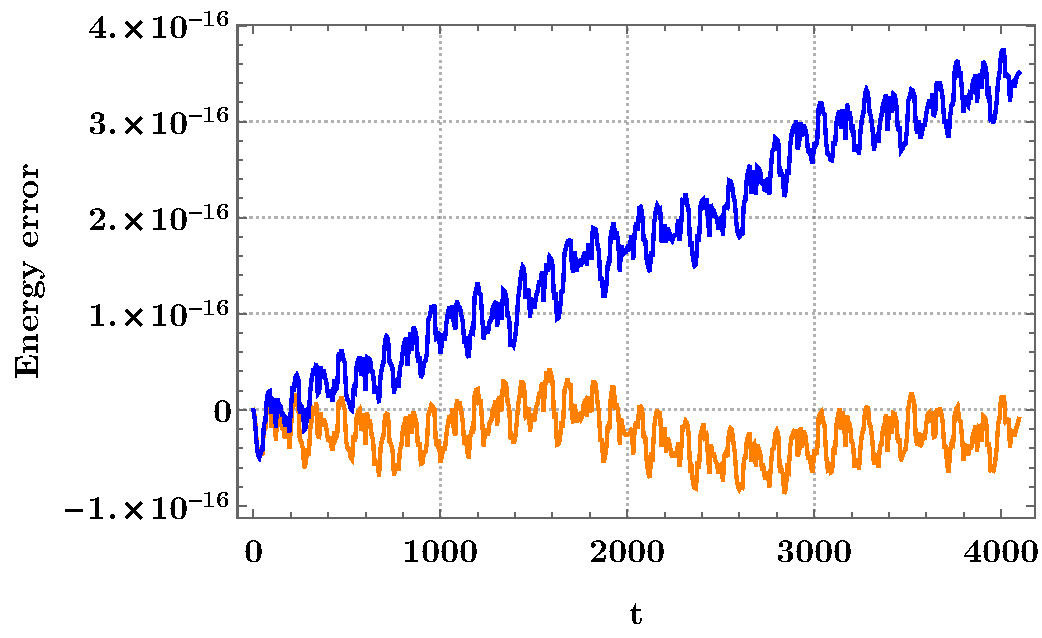
\includegraphics[width=.4\textwidth]{Fig2N}}
&
\subfloat[$k=0$ energia errorearen desbideratze estandarra]
{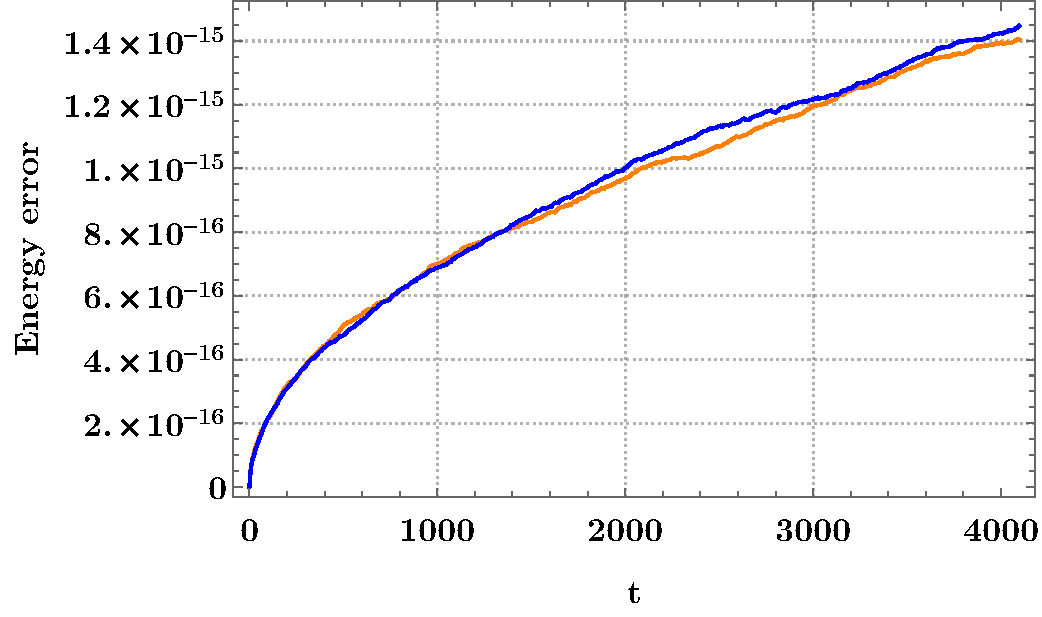
\includegraphics[width=.4\textwidth]{Fig3N}}
\\
\subfloat[$k=2^{10}$ energia errorrearen batezbestekoa]
{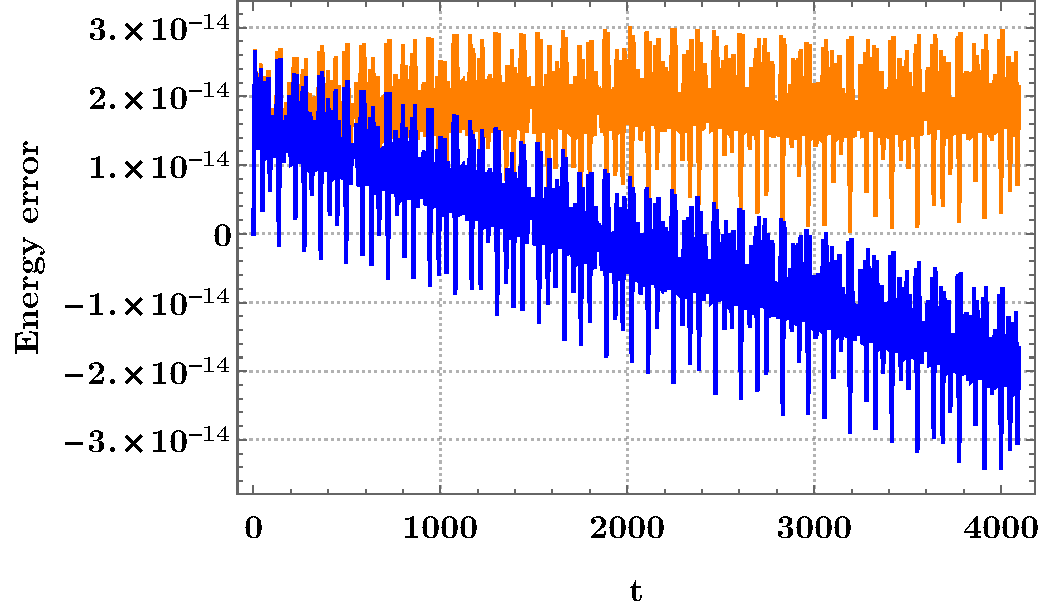
\includegraphics[width=.4\textwidth]{Fig4N}}
&
\subfloat[$k=2^{10}$ energia errorearen desbideratze estandarra]
{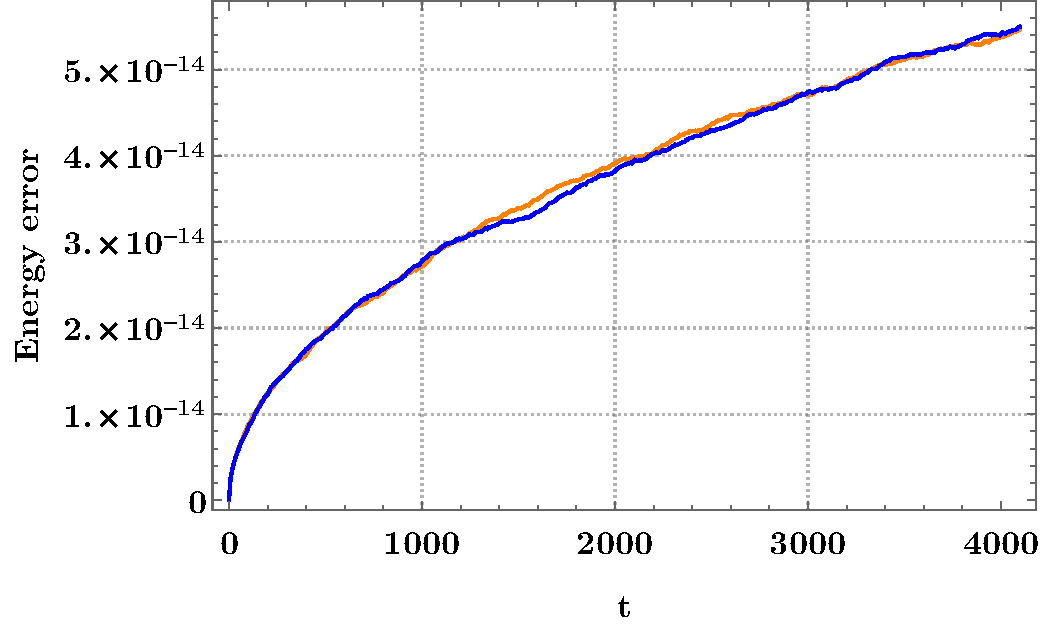
\includegraphics[width=.4\textwidth]{Fig5N}}
\\
\subfloat[$k=2^{12}$ energia errorrearen batezbestekoa]
{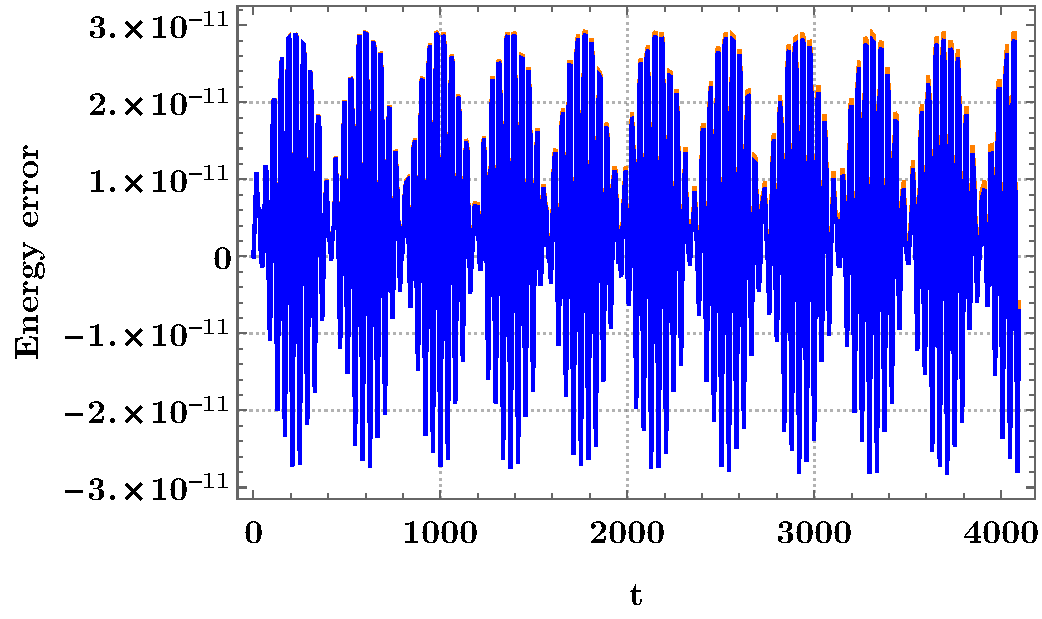
\includegraphics[width=.4\textwidth]{Fig6N}}
&
\subfloat[$k=2^{12}$ energia errorearen desbideratze estandarra]
{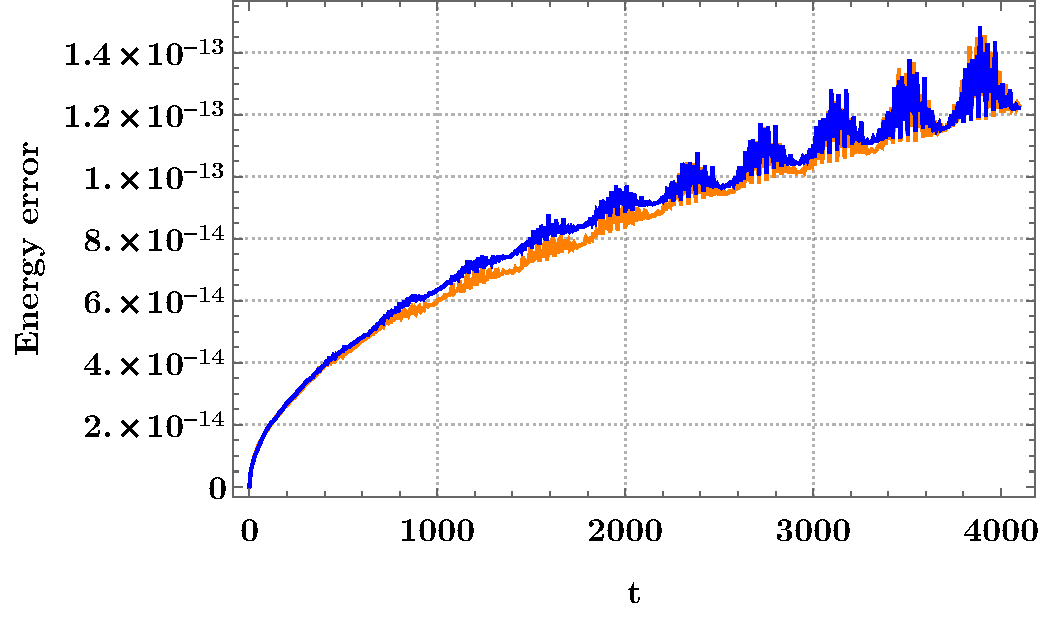
\includegraphics[width=.4\textwidth]{Fig7N}}
\end{tabular}
\caption[Biribiltze errorearen azterketa]{\small Energia errorearen batezbestekoaren (ezkerrean) eta desbideratze estandarraren  eboluzioa (eskuinean), puntu-finkoaren inplementazioa (urdinez), eta  Newton inplementazioa (laranjaz). $k=0$ problema ez-zurruna (a,b), $k=2^{10}$ lehen problema zurruna (c,d) eta $k=2^{12}$ bigarren problema zurruna (e,f)}
\label{fig:plot3}
\end{figure}


\subsection{Puntu-finkoa versus Newton iterazioa}


\ref{tab:fp1} taulan, $k$ parametroaren lau balioetarako, bi inplementazioen eraginkortasunaren adierazle nagusienak laburtu ditugu.

\begin{table}[h!]
\caption[Puntu-finkoa versus Newton iterazioa] 
{\small}
\label{tab:fp1}       % Give a unique label
\centering
{%
\begin{tabular}{ l l l l l } 
 \hline
%                 &  \multicolumn{2}{c}{FPIEA}  & \multicolumn{2}{c}{DP} & \multicolumn{2}{c}{Hairer} \\
\\
 $k$               & $0$  & $2^3$ & $2^6$ & $2^8$ \\
 $E_0$           & $-14.39$  & $-5.75$ & $-5.64$ & $-5.64$ \\ 
\\
 \hline
\\
 Fixed-points it.&           &         &         &         \\
 \cline{1-1}     &           &         &         &         \\
 Elapsed-time (sec.)    & $10$      & $12$    & $19$    & $51$    \\ 
 It. per step    & $8.58$    & $11.1$  & $22.$  & $64.2$  \\
 Energy          & $2.96\times 10^{-15}$ & $1.81\times 10^{-14}$ & $2.94\times 10^{-11}$ & $6.33\times 10^{-5}$ \\
 \\
 Newton it.            &           &         &         &         \\
 \cline{1-1}           &           &         &         &         \\
 Elapsed-time (sec.)   & $18$      & $20$    & $19$    & $18$     \\
 It. per step          & $5.09$    & $5.53$  & $5.58$  & $5.01$   \\
 L. solves per step    & $11.37$   & $12.92$  & $12.72$  & $11.04$ \\
 Energy                & $1.6\times 10^{-15}$ & $1.74\times 10^{-14}$ & $2.94\times 10^{-11}$ & $6.33\times 10^{-5}$ \\   
 \\  
   \hline
 \end{tabular}}
\end{table}

Eraginkortasuna neurtzeko, bi inplementazioen exekuzio sekuentzialen CPU-denborak  konparatu ditugu. Horrez gain, bi inplementazioen urratseko iterazioen batezbestekoak (It. per step) alderatu ditugu eta Newton inplementazioan, urratseko sistema linealen ebazpenen batezbestekoa (L.solves per step) eman dugu. Zenbakizko soluzioaren doitasuna neurtzeko, energiaren errore erlatiboaren maximoa eman dugu,
\begin{equation*}
\max | \frac{E(t_n)-E(t_0)}{E(t_0)}|, \ \  t_n=t_0+nh, \ \ n=1,2,\dots
\end{equation*} 

$k$ balio txikienetarako, puntu-finkoaren inplementazioa Newton inplementazioa baino eraginkorragoa da. Baina, pendulu bikoitzaren zurruntasun maila handitzen dugunean, puntu-finkoaren iterazio kopurua gero eta handiagoa den bitartean, Newton inplementazioaren iterazio kopurua mantendu egiten den, eta $k$ handietan txikitu ere bai. Beraz, zurruntasuna handitzen dugunean, Newton inplementazioa gero eta eraginkorragoa bilakatzen da. $k=2^{18}$ baliotik aurrera, puntu-finkoak ez du konbergitzen eta Newton inplementazioak, antzeko iterazio kopuruarekin konbergitzen du.

 
%\small{Percentage of steps that reach a computational fixed-point and the number of fixed-point iterations per step for the computations of  double pendulum stiff problem}



\section{Laburpena}

IRK metodoen Newton sinplifikatuaren iterazioen ekuazio-sistema, modu eraginkorrean askatzeko inplementazioa proposatu dugu. Newtonen iterazioan oinarritutako IRK metodoaren inplementazio berria aurkeztu dugu eta inplementazio honen biribiltze errorearen hedapena egokia dela baieztatu dugu. Problema zurrunetarako, Newton sinplifikatuaren iterazioa, puntu-finkoaren iterazioa baino eraginkorragoa dela ikusi dugu.

Newtonen iterazioan oinarritutako IRK metodoen inplementazioen inguruko lan hauek \cite{Butcher1976,Hairer2006} gomendatuko ditugu .

Azkenik, aipatu nahi dugu, atal honen edukiak \href{http://link.springer.com/journal/11075}{Numerical Algorithms} aldizkarian publikatutako \cite{Antonana2017a} artikuluan aurki daitezkeela eta inplementazioaren kodea, helbide honetan   \url{https://github.com/mikelehu/IRK-Newton} eskuragarri jarri dugula.
